\documentclass[]{scrreprt}
\KOMAoptions{fontsize=14pt}

\usepackage{amsmath,amsfonts,amssymb,amsthm,mathtools} % AMS

\usepackage{hyperref}       % hyperref
\hypersetup{				% settings
	unicode=true,           % non-latin letters
	pdftitle={Practical application of the Wilcoxon-Mann-Whitney test in valuation
},   % heading
	pdfauthor={K. A. Murashev},      % Author
	pdfsubject={Wilcoxon-Mann-Whitney test},      % Scope
	pdfcreator={K. A. Murashev}, % Creator
	pdfproducer={K. A. Murashev}, % Producer
	pdfkeywords={Wilcoxon-Mann-Whitney test, U-test} % Keywords
	colorlinks=true,       	% false: links in frames; true: coloured links
	linkcolor=red,          % internal links
	citecolor=green,        % bibliography links
	filecolor=magenta,      % file links
	urlcolor=blue           % URL links
}

\usepackage{url}

\usepackage{babel}

% work with images
\usepackage{graphicx}
\graphicspath{{Images/}}

% work with tables
\usepackage{array, tabularx, tabulary, booktabs, xtab} % additional forms of tables
\usepackage{longtable}  % long tables
\usepackage{multirow} % merge rows

% work with bibliography
\usepackage[backend=biber,bibencoding=utf8,sorting=ynt,maxcitenames=5,sortupper=true,date=iso]{biblatex}

% set the depth of table of contents
\setcounter{tocdepth}{8}

% work with scripts
\usepackage {listings}
\lstloadlanguages{[Latex]Tex, bash, R, Python, SQL}
\lstset{extendedchars=true , % additional symbols
frame=tb, % top & bottom frames
commentstyle=\itshape , % font for comments
stringstyle =\ttfamily % font for 'strings'
keywordstyle=\color{blue} % color for keywords
}

% connecting the automated bibliography package
\usepackage[backend=biber,bibencoding=utf8,sorting=ynt,maxcitenames=5,sortupper=true,date=iso]{biblatex} 

% add sources for bibliography
\addbibresource{/home/kaarlahti/TresoritDrive/Methodics/My/AI_for_valuers/Book/AI_for_valuers_book/Basic_principles.bib}
\addbibresource{/home/kaarlahti/TresoritDrive/Methodics/My/AI_for_valuers/Book/AI_for_valuers_book/LaTeX.bib}
\addbibresource{/home/kaarlahti/TresoritDrive/Methodics/My/AI_for_valuers/Book/AI_for_valuers_book/Mathstat.bib}
\addbibresource{/home/kaarlahti/TresoritDrive/Methodics/My/AI_for_valuers/Book/AI_for_valuers_book/Murashev.bib}
\addbibresource{/home/kaarlahti/TresoritDrive/Methodics/My/AI_for_valuers/Book/AI_for_valuers_book/Python.bib}
\addbibresource{/home/kaarlahti/TresoritDrive/Methodics/My/AI_for_valuers/Book/AI_for_valuers_book/R.bib}
\addbibresource{/home/kaarlahti/TresoritDrive/Methodics/My/AI_for_valuers/Book/AI_for_valuers_book/RussianLaws.bib}
\addbibresource{/home/kaarlahti/TresoritDrive/Methodics/My/AI_for_valuers/Book/AI_for_valuers_book/Sci&Tech.bib}
\addbibresource{/home/kaarlahti/TresoritDrive/Methodics/My/AI_for_valuers/Book/AI_for_valuers_book/Valuation.bib}
\addbibresource{/home/kaarlahti/TresoritDrive/Methodics/My/AI_for_valuers/Book/AI_for_valuers_book/ValuationStandards.bib}
\addbibresource{/home/kaarlahti/TresoritDrive/Methodics/My/AI_for_valuers/Book/AI_for_valuers_book/ZHZL.bib}

\usepackage{bbm} % indicator function

\newcommand{\github}{
	{%
		
\includegraphics[width=3ex,height=3ex,keepaspectratio]{github-seeklogo.pdf}
}
}


% Title Page
\title{Practical application of~the~Wilcoxon-Mann-Whitney test in~valuation.}
\subtitle{Selection of~attributes as~pricing factors based on~the~principle of~unbiased estimates}
\author{\href{https://www.facebook.com/groups/1977067932456703}{K.~A.~Murashev}}

\begin{document}
\maketitle
%
\lstset{language=Python,
	basicstyle=\ttfamily,
	keywordstyle=\color{Blue}\ttfamily,
	stringstyle=\color{Red}\ttfamily,
	commentstyle=\color{Emerald}\ttfamily,
	morecomment=[l][\color{Magenta}]{\#},
	breaklines=true,
	breakindent=0pt,
	breakatwhitespace,
	columns=fullflexible,
	showstringspaces=false
}
%	
\begin{abstract}
	In~their practice appraisers often face the~need to~take into account differences in~quantitative and~qualitative characteristics of~objects. In~particular, one of~the~standard tasks is~to~determine the~attributes that influence the~cost (so-called "pricing factors") and~to~separate them from the~attributes that do~not or~cannot be~determined.
	
	Subjective selection of~attributes taken into account in~determining the~value is~widespread in~valuation practice. In~this case, specific quantitative indicators of~the~impact of~these attributes on~the~cost are~often taken from the~so-called "reference books". While not~denying the~speed and~low cost of~this approach, it~should~be recognized that only data directly observed in~the open markets is~a~reliable basis for~a~value judgment. The priority of~such data over other data, in~particular those obtained by~expert survey, is~enshrined, among others, in~\href{https://www.rics.org/uk/upholding-professional-standards/sector-standards/valuation/red-book/red-book-global/}{RICS Valuation --- Global Standards 2022}~\cite{RVGS-2022}, \href{https://www.rics.org/uk/upholding-professional-standards/sector-standards/valuation/red-book/international-valuation-standards/}{International Valuation Standards 2022}~\cite{IVS-2022}, as~well as~in~\href{http://eifrs.ifrs.org/eifrs/bnstandards/en/IFRS13.pdf}{IFRS~13 "Fair Value Measurement"}~\cite{IFRS-13}. Therefore, we~can say that mathematical methods for~analyzing data from the open market are the~most reliable means of~interpreting market information used in~market research and~predicting the~value of~individual objects.
	
	The aim of~this work is~to~justify the~necessity and~possibility of~using a~rigorous mathematical Wilcoxon--Mann--Whitney test, which allows us~to~answer the~question about the~necessity of~taking into account the~binary attribute as~a~price-generating factor. Instead of~the~judgmental approach, which is~most commonly used by~appraisers in~selecting the~attributes to~be considered in~appraisal, this paper proposes the~idea of~prioritizing the~measuring approach based on~the~results of~a~mathematical test that allows to~draw a~conclusion about the~importance or~otherwise of~the~binary attribute influence on~the~value. It~should~be noted that despite the~fact that the~statistical test under consideration belongs to~frequentist statistics, it, through its~connection to~ROC analysis and~AUC, is~related to~modern machine learning methods, which will~be discussed later in~the~text of~this material. The~presence of~this relationship and~elements of~Bayesian statistics seems particularly interesting and~promising from the~point of~view of~introducing machine learning and~data analysis methods into the~everyday practice of~appraisers.
	
	Users should have some general math background and~basic Python and~R programming skills to~understand and~practice all of~the material in~the~text, but~lack of~that knowledge and~skill is~not~a~barrier to~learning most of~the~material and~implementing the~test in~the~spreadsheet that comes with it.
	
	The material consists of~four blocks:
	\begin{itemize}
		\item a~description of~the~Wilcoxon--Mann--Whitney test (hereafter "U-test"), its probabilistic meaning, and~its relationship to~other mathematical methods;
		\item a~practical implementation of~the~U-test in~a~spreadsheet on~an~example of~test random data;
		\item practical implementation of~the~U-test on~the~real data of~the~residential real estate market of~St.~Petersburg agglomeration by~means of~Python programming language, the~purpose of~the~analysis was~to~check the~significance of~the~difference in~the~unit price between the~objects located in~the~urban and~suburban parts of~the~agglomeration;
		\item practical implementation of~the~U-test on~real data of~residential real estate market of~Almaty by~means of~R programming language, the~purpose of~the~analysis was~to~check the~significance of~difference in~unit price between the~objects sold without demountable improvements and~the~objects sold with them.
	\end{itemize}
	The~current version of~this material, its source code, Python and~R scripts, and~the~spreadsheet are~in~the~repository on~the GitHub portal and~are~available at~the~\href{https://github.com/Kirill-Murashev/AI_for_valuers_book/tree/main/Parts-Chapters/Mann-Whitney-Wilcoxon}{permanent link}~\cite{Murashev:u-test}.
	
	This material and~all of~its~appendices are~distributed under the~terms of~the~\href{https://creativecommons.org/licenses/by-sa/4.0/}{cc-by-sa-4.0} license~\cite{cc-by-sa-4.0}.
\end{abstract}	
%
\tableofcontents
\listoftables
\listoffigures
\lstlistoflistings
%	
\chapter{Technical details}
This material, as~well as~the~appendices to~it, are available at~\href{https://github.com/Kirill-Murashev/AI_for_valuers_book/tree/main/Parts-Chapters/Mann-Whitney-Wilcoxon}{permanent link}~\cite{Murashev:u-test}. The~source code for~this work was~created~using the~language~\href{https://www.ctan.org/}{\TeX}~\cite{TeX:site} with~a~set of~macro extensions~\href{https://www latex-project.org/}{\LaTeXe}~\cite{LaTeX:site}, distribution~\href{https://www.tug.org/texlive/}{TeXLive}~\cite{TeXLive:site} and~Editor~\href{https://www.texstudio.org/}{TeXstudio}~\cite{TeXstudio:site}. The~spreadsheet calculation was~done with \href{https://www.libreoffice.org/discover/calc/}{LibreOffice Calc}~\cite{LO:Calc} (Version: 7.3.4. 2 / LibreOffice Community Build ID: 30(Build:2); CPU threads: 4; OS: Linux 5.11; UI render: default; VCL: kf5 (cairo+xcb) Locale: en-US (en\_US.UTF-8); UI: en-US Ubuntu package version: 1:7.3.4~rc2-0ubuntu0.20.04.1~lo1; Calc: threaded). The~calculation in~\href{https://www.r-project.org/}{R}~\cite{R_language} (version 4.2.1 (2022-06-23) -- "Funny-Looking Kid") was~done~using an~IDE~\href{https://www.rstudio.com/}{RStudio} (RStudio 2022. 02.3+492 "Prairie Trillium" Release (1db809b8, 2022-05-20) for Ubuntu Bionic; Mozilla/5.0 (X11; Linux x86\_64); AppleWebKit/537.36 (KHTML, like Gecko); QtWebEngine/5.12.8; Chrome/69.0.3497.128; Safari/537.36)~\cite{RStudio:official_site}. The~calculation in~\href{https://www.python.org/}{Python}~(Version~3.9.12)~\cite{Python:site} was~performed using the~development environment~\href{https://jupyter.org}{Jupyter Lab} (Version 3.4.2)~\cite{Jupyter:site} and~IDE \href{https://www.spyder-ide.org/}{Spyder} (Spyder version: 5.1.5 None* Python version: 3.9.12 64-bit * Qt version: 5.9.7 * PyQt5 version: 5.9.2
* Operating System: Linux 5.11.0-37-generic)~\cite{Spyder:site}. The~graphics used in~the~subsection \ref{U-test-spreadsheet} were prepared using \href{Geogebra:official-site}{Geogebra}~(Version 6.0.666.0-202109211234)~\cite{Geogebra:official-site}. The~following values were used in~this material as~well as~in~most of~the~works in~the~series:
\begin{itemize}
	\item significance level: $\alpha = 0.05$;
	\item confidence interval: $Pr = 0.95$;
	\item initial position of the pseudo-random number generator: $seed=19190709$.
\end{itemize}
A~dot is~used as~a~decimal point. Most of~the~mathematical notations are~written as~they are~used in~English-speaking circles. For~example, a~tangent is~written as~$\tan$, not~$\tg$. The~results of~statistical tests are~considered significant when
\begin{equation}\label{eq:significance}
p \leq \alpha.
\end{equation}
This decision is~based, in~part, on~the~results of~the~discussion that took place on~\href{researchgate.net}{researchgate.net}~~\cite{RG:p-equals-alpha}.
%
\chapter{Subject of~research}
When working with market data, the~appraiser is~often faced with the~task of~testing the~hypothesis of~whether a~quantitative, ordinal or~nominal attribute has~a~significant effect on~the~price. Real estate market analysts, developers, realtors, employees of~collateral departments of~banks, leasing and~insurance companies, tax inspectors and~other specialists have a~similar task. At~the~same time, it~is~often impossible to~collect large amounts of~data that would allow a~wide range of~machine learning methods to~be~applied. In~some cases appraisers consciously narrow the~area of~data collection to~the~narrow market segment, resulting in~only very small samples of~less than thirty observations at~their disposal. In~this case, the~price data most often has~a~distribution that differs from the~normal one. In~this case, a~rational solution is~to~use U-test. Let~us formulate the~problem:
\begin{itemize}
	\item suppose that we~have two samples of~unit prices for~commercial premises, some of~which have some attribute (e.\,g., having a~separate entrance) and~some of~which do~not;
	\item it~is~necessary to~determine whether the~presence of~this feature has a~significant impact on~the~unit value of~this type of~real estate or~not.
\end{itemize}
At~first glance, according to~established practice, an~appraiser can simply subjectively recognize some attributes as~significant and~others as~not, and~then accept the~adjustment values for~differences in~these attributes from the~reference books. However, as~mentioned above, this approach is~hardly considered best practice because it~lacks any~market analysis. Also, in~that case, it~is~unlikely that such work is~of~any~serious value at~all.

Instead, it~is~possible to~use random samples of~market data and~apply mathematical analysis to~them, allowing scientific and evidence-based conclusions to~be~drawn about the~significance of~a~particular attribute's impact on~value. The~data used in~this paper to~perform the~U-test using Python and~R are~real market data, some of~which were collected by~the author through web scraping and some provided by~colleagues for~the~analysis. The~attached spreadsheet is~set~up so~that test raw data can~be generated in~a~pseudo-random fashion.

The~subject of~this paper is~the~nonparametric Wilcoxon-Mann-Whitney test, specifically designed for~samples that have a~distribution other than normal. This circumstance is~important because the~price data that appraisers deal with most often have this distribution, which excludes the~possibility of~applying the~parametric t-criterion and~z-criterion. In~addition, the~test under consideration is~of~great interest because it~has a~connection to~machine learning methods through AUC, the~calculation of~which through the~formula provided in~the~test framework gives a~value equal to~that calculated by~ROC analysis. Thus, the~study of~the~U-test paves the~way for~a~further dive into the~world of~machine learning, which is~entering many areas of~human activity and~will significantly change the~field of~value estimation in~the~foreseeable future.

The~material contains a~description of~the~test and~instructions for~performing it, sufficient in~the~author's opinion for~its~demonstrable use in~the~estimation process.
%
\chapter{Basic information about the~test}
\section{Assumptions and~formalization of~hypotheses}
First of~all, it~should~be said that, in~spite of~the~stated common name, it~is~more correct to~speak of~two tests:
\begin{itemize}
	\item \href{http://www.machinelearning.ru/wiki/index.php?title=Критерий_Уилкоксона_двухвыборочный}{Wilcoxon rank-sum test} developed by~Frank Wilcoxon in~1945~\cite{MLRU:Wilcoxon-test};
	\item \href{http://www.machinelearning.ru/wiki/index.php?title=Критерий_Уилкоксона-Манна"--~Уитни}{Mann--Whitney~U-test} which is~a~further development of~the~aforementioned criterion developed by~Henry Mann and~Donald Whitney in~1947~\cite{MLRU:Mann-Whitney}.
\end{itemize}
Looking ahead we~can say that the~statistics of~these criteria are~linearly related and~their p-values are~almost the~same which from a~practical point of~view allows us to~talk about variations of~one test rather than two separate tests. This paper uses the~common name throughout the~text, as~well as~a~shortened version of~"U-test" which historically refers to~the~Mann-Whitney test. Some authors\cite{Kobzarq-prikl-mathstat} recommend using the~Wilcoxon rank-sum test when there are~no~assumptions about variance, and the~Mann-Whitney U-test when variance of~the~two samples are~equal. However, the~experimental data indicate that the~Wilcoxon rank-sum test and~Mann-Whitney U-test values are~essentially the~same when the~variance of~the~samples is~significantly different. Adhering to~the~KISS principle~\cite{KISS-principle} underlying the~entire series of~publications, the~author concludes that a~unified approach is~possible. Also remember that the~Wilcoxon signed-rank test is~a~separate test designed to~analyze differences between two matched samples, whereas the~Mann-Whitney U-test discussed in~this paper is~designed to~work with two independent samples.

Suppose that there are~two samples:
\begin{equation*}
x^{m} = (x_{1},x_{2},\ldots,x_{m}), x_{i} \in \mathbb{R};\quad y^{n} = (y_{1},y_{2},\ldots,y_{n}), y_{i} \in \mathbb{R} \quad: m \leq n.
\end{equation*}
%
\begin{itemize}
	\item Both samples are~simple and~random (i.e., \href{https://en.wikipedia.org/wiki/Simple_random_sample}{SRS}~\cite{Wiki:SRS}), the~combined sample is~independent.
	\item The~samples are~taken from unknown continuous distributions \textit{F(x)} and~\textit{G(y)}, respectively.
\end{itemize}
%
\begin{description}
	\item[Simple random sample~(SRS) ---] is~a~subset of~individuals (\emph{a~sample}) chosen from a~larger set (\emph{a~population}) in~which a~subset of~individuals are~chosen randomly, all with the~same probability. It~is~a~process of~selecting a~sample in~a~random way. In~\textbf{SRS}, each subset of~\textit{k}~individuals has~the~same probability of~being chosen for~the~sample as~any~other subset of~\textit{k}~individuals.A~simple random sample is~an~unbiased sampling technique. Equivalent definition: a~sample ${\textstyle x^{m} = (x_{1},x_{2},\ldots,x_{m})}$ is~simple if~the~values~${\textstyle (x_{1},x_{2},\ldots,x_{m})}$ are~realizations of~\textit{m} independent equally distributed random variables. In~other words, the~selection of~observations is~not~only random but also does not~imply any~special selection rules (e.g., choosing every 10th observation).
\end{description}
%
\begin{description}
	\item[The~U-test ---] is~a~nonparametric criterion to~test the~null hypothesis that for~randomly chosen from~two samples of~observations~$x \in X$ and~$y \in Y$ the probability that~\textit{x} is~greater than \textit{y} is~equal to~the~probability that~\textit{y} is~greater than~\textit{x}. In~mathematical language, the~null hypothesis is~written as~follows
	\begin{equation}\label{eq:U-test-null-hypothesis}
	H_{0}:P\{x<y=\frac{1}{2}\}.
	\end{equation}
	For~the~test's own consistency, an~alternative hypothesis is~required, which is~that the~probability that the~value of~a~characteristic of~observation from~\textit{X} is~greater than that of~observation from~\textit{Y} differs upward or~downward from the~probability that the~value of~a~characteristic of~observation from~\textit{Y} is~greater than that of~observation from~\textit{X}. In~mathematical language, the~alternative hypothesis is~written as~follows
	\begin{equation}\label{eq:U-test-alt-hypothesis}
	H_{1}:P\{x<y\} \neq P\{y<x\} \vee P\{x<y\} + 0.5 \cdot P\{x=y\} \neq 0.5.
	\end{equation}
\end{description}
According to~the~basic concept of~the~U-test, if~the~null hypothesis is~true, the~distribution of~the~two samples is~continuous; if~the~alternative hypothesis is~true, the~distribution of~one sample is~stochastically greater than the~distribution of~the~other. In~this case, it~is~possible to~formulate a~number of~null and~alternative hypotheses for~which this test will give a~correct result. His~most extensive generalization lies in~the~following assumptions:
\begin{itemize}
	\item the~observations in~both samples are~independent;
	\item the~data type is~at~least ranked, i.\,e., with respect to~any two observations you can tell which one is~greater;
	\item the~null hypothesis assumes that the~distributions of~the~two samples are equal;
	\item the~alternative hypothesis assumes that the~distributions of~the~two samples are unequal.
\end{itemize}
With a~stricter set of~assumptions than those given above, for~example the~assumption that the~distribution of~the~two samples is~continuous if~the~null hypothesis is~valid and that the~distribution of~the~two samples has a~shift  in~the~distribution if~the~alternative one is~valid i.\,e.~$f_{1}(x)=f_{2}(x+\sigma)$,  we~can say that the~U-test is~a~test for~the~hypothesis of~equality of~medians. In~this case, the~U-test can~be interpreted as~a~test of~whether Hodges--Lehman's estimate of~the~difference in~central tendency measures differs from zero. In~this situation, the~Hodges--Lehman estimate is~the median of~all possible values of~differences between the~observations in~the~first and second samples. However, if~both the~variance and the~shape of~the~distribution of~the~two samples differ, the~U-test cannot correctly test the~medians. Examples can~be shown where the~medians are~numerically equal and the~test rejects the~null hypothesis because of~the~small p-value. Thus, a~more correct interpretation of~the~U-test is~to~use~it to~test the~\href{http://www.machinelearning.ru/wiki/index.php?title=Гипотеза_сдвига}{shift hypothesis}~\cite{MLRU:shift-hypothesis}.
\begin{description}
	\item[Shift hypothesis ---] is~a~statistical hypothesis often considered as~an~alternative to~the~hypothesis of~complete homogeneity of~samples. Let~us have two samples of~data. Let~us also give two random variables~\textit{X} and~\textit{Y}, which are~distributed as~elements of~these samples and have distribution functions~\textit{F(x)} and~\textit{G(y)}, respectively. In~these terms, the~shift hypothesis can~be written as~follows
	\begin{equation}\label{eq:shift-hypothesis}
	H:F(x)=G(x+\sigma)\ : \forall x,\ \sigma \neq 0.
	\end{equation}
\end{description}
In~this case, the~U-criterion is~valid regardless of~the~characteristics of~the~samples.

Simply put, the~essence of~the~U-test is~that it~allows~us to~answer the~question of~whether there~is a~significant difference in~the~value of~the~quantitative attribute of~the~two samples. With regard to~valuation, we~can say that the~use of~this test helps to~answer the~question of~whether it~is~necessary to~take into account one or~another attribute as~a~price-generating factor. It~follows from the~above that by~default we~are talking about a~two-sided test. In~practice, this means that the~test does~not give a~direct answer to~the~question, for~example: "Is~there a~significant excess of~the~unit value of~premises with a~separate entrance to~the~premises that do~not have it. At~the~same time, there~are also one-sided realizations that allow~us to~answer the~question about the~sign of~the~difference in~the~value of~the~attribute in~the~two samples.

In~addition to~the~above requirements for~the~samples themselves, the~conditions for~applying the~U-test are:
\begin{itemize}
	\item the~distribution of~quantitative attribute values of~samples is~different from normal (otherwise it~is advisable to~use parametric Student's t-test or~z-test for~independent samples).
	\item at~least three observations in~each sample, it~is~allowed to~have two observations in~one of~the~samples, provided that there~are at~least five in~the~other sample.
\end{itemize}
To~summarize the~above, there~are three variants of~the~null hypothesis, depending on~the~level of~rigor outlined in~the~table below~\ref{tab:nul-hypothesis-variants}.
\begin{table}[ht]
	\caption{Variants of~the~null hypothesis when using the~U-test in~valuation.}\label{tab:nul-hypothesis-variants}
	\centering
	\begin{tabularx}{\textwidth}{p{0.25\linewidth} p{0.7\linewidth}} 
		\hline
		Type of~hypothesis&Formulation\\
		\hline
		Scientific&The~two samples are~completely homogeneous, i.\,e.~they belong to~the~same distribution, there~is no~shift and the~estimate made for~the~first sample is~unbiased for~the~second one.\\
		\hline
		Practical&The~medians of~the~two samples are~equal to~each other.\\
		\hline
		Set forth in~terms of~valuation&The~difference in~the~attribute between the~two samples of~object-analogues is~not~significant, its accounting is~not required and this attribute is~not a~pricing factor.\\
		\hline
	\end{tabularx}
\end{table}
%
\section{Test implementation}
\subsection{Test statistic}
Suppose that~the elements $x_{1},\ldots,x_{n}$ represent a~simple independent sample from~$X \in \mathbb{R}$, and~the elements $y_{1},\ldots, y_{n}$ represent a~simple independent sample from $Y \in \mathbb{R}$ and the~samples are~independent of~each other. Then the~relevant U-statistic is~defined as~follows:
\begin{equation}\label{eq:U-statistic-base-formula}
\begin{aligned}
U&=\sum_{i=1}^{m} \sum_{j=1}^{n} S (x_{i},y_{j}),\\
&\text{при}\\
S(x,y)&=
\begin{cases}
1,\quad \text{если}\ x>y,\\
\frac{1}{2},\quad \text{если}\ x=y,\\
0,\quad \text{если}\ x<y.
\end{cases}
\end{aligned}
\end{equation}
%
\subsection{Calculation methods}
The~test involves calculating a~statistic usually called the~U-statistic whose distribution is~known if~the~null hypothesis is~true. When working with very small samples, the~distribution is~specified tabularly; when the~sample size is~more than twenty observations, it~is~approximated quite well by~the~normal distribution. There are~two methods of~calculating U-statistics: manual calculation using the~formula \ref{eq:U-statistic-base-formula} or~using a~special algorithm. The~first method, due~to its~labor-intensive nature, is~only suitable for~very small samples. The~second method can~be formalized as~a~step-by-step set of~instructions and will~be described below.
\begin{enumerate}
	\item You must construct a~common variation series for~the~two samples and then assign a~rank to~each observation, starting with one for~the~smallest of~them. If~there are~ties, i.\,e. groups of~repeating values (such a~group can~be, e.\,g., only two equal values), each observation from such a~group is~assigned a~value equal to~the~median of~the~group ranks before adjustment (for example, in~the~case of~a~variation series (\textit{3, 5, 5, 5, 5, 8}) the~ranks before adjustment are~(\textit{1, 2, 3, 4, 5, 6}) after --- (\textit{1, 3.5, 3.5, 3.5, 3.5, 6}).
	\item It~is necessary to~calculate the~sums of~the~ranks of~the~observations of~each sample, denoted as~${R_{1},\ R_{2}}$ respectively. In~this case, the~total sum of~ranks can~be calculated by~the~formula
	\begin{equation}\label{eq:common-R}
	R = \frac{N(N+1)}{2},
	\end{equation}
	where~\textit{N} ---the~total number of~observations in~both samples.
	%
	\item Next, we~calculate the~U-value for~the~first sample:
	\begin{equation}\label{eq:U1}
	U_{1}=R_{1}-\frac{n_{1}(n_{1}+1)}{2},
	\end{equation}
	where $R_{1}$ ---the~sum of~ranks of~the~first sample, $n_{1}$ --- the~number of~observations in~the~first sample.
	%
	\item The~U-value for~the~second sample is~calculated in~the~same way:
	\begin{equation}\label{eq:U2}
	U_{2}=R_{2}-\frac{n_{2}(n_{2}+1)}{2},
	\end{equation}
	where $R_{2}$ ---the~sum of~ranks of~the~second sample, $n_{2}$ --- the~number of~observations in~the~second sample.
	
	From the~above formulas it~follows that
	\begin{equation}\label{eq:U1-U2-relation}
	U_{1}+U_{2} = R_{1}-\frac{n_{1}(n_{1}+1)}{2} + R_{2}-\frac{n_{2}(n_{2}+1)}{2}.
	\end{equation}
	It~is~also known that
	\begin{equation}\label{eq:R-N-relation}
	\begin{cases}
	R_{1}+R_{2}=\dfrac{N(N+1)}{2}\\
	N=n_{1}+n_{2}.
	\end{cases}
	\end{equation}
	Then
	\begin{equation}\label{eq:check-U-value}
	U_{1}+U_{2}=n_{1}n{2}.
	\end{equation}
	Using this formula as~a~control ratio can~be useful for~checking the~correctness of~calculations in~a~spreadsheet processor.
	%
	\item From the~two values of~$U_{1},\ U_{2}$ in~all cases we~choose the~smaller which will~be the~U-statistic and~used in~further calculations. Let~us denote it~as~\emph{U}.
\end{enumerate}
%
\subsection{Interpretation of~the~result}
For~a~correct interpretation of~the~test result it~is necessary to~specify:
\begin{itemize}
	\item size of each sample;
	\item values of~the~measure of~central tendency for~each sample (given the~nonparametric nature of~the~test, the~median appears to~be the~appropriate measure of~central tendency);
	\item the~value of~the~U-statistic itself;
	\item the~\href{https://en.wikipedia.org/wiki/Effect_size#Common_language_effect_size}{CLES} index~\cite{Wiki:CLES} the~value of~which is~equivalent to~the~AUC and~$\rho$-statistic;
	\item \href{https://en.wikipedia.org/wiki/Effect_size#Rank-biserial_correlation}{rank-biserial correlation coefficient~(RBC)}~\cite{Wiki:rank-biserial-correlation};
	\item the~accepted level of~significance (usually 0.05);
	\item the~calculated p-value.
\end{itemize}
The~concept of~U-statistic was discussed earlier and most of~the~other indicators are widely known and do~not require any particular consideration. 
\subsubsection{CLES = $\rho$-statistic = AUC}
First of~all, it~must~be said that all of~these indicators are~equivalent to~each other. Thus
\begin{equation}\label{eq:AUC=CLES}
CLES = f = AUC_{1} = \rho.
\end{equation}
\paragraph{Common language effect size~(CLES)}
\begin{description}
	\item[Common language effect size~(CLES) ---] is the~probability that the~value of~a~randomly chosen observation from the first sample is greater than the~value of~a~randomly chosen observation from the second sample. This indicator is~calculated by~the~formula
	\begin{equation}\label{eq:CLES}
	CLES = \frac{U_{1}}{n_{1}n_{2}}.
	\end{equation}
	The designation \emph{f~(favorable)} is~often used instead of~\emph{CLES}. This sample value is~an~unbiased estimate of~the~value for~the~entire population of~objects belonging to~the~set.	
\end{description}
It~should~be noted that the~value and meaning of~this indicator is~equivalent to~the~value and meaning of~the ~\href{https://en.wikipedia.org/wiki/Receiver_operating_characteristic}{AUC}\cite{Wiki:ROC}. Thus, we~can say that this indicator characterizes the~quality of~ the~U-test as~a~binary classifier.
\begin{equation}\label{eq:AUC}
CLES = f = AUC_{1} = \frac{U_{1}}{n_{1}n_{2}}.
\end{equation}
The~relationship between the~U-statistic and~AUC is~discussed in~\ref{U-AUC}.
%
\paragraph{$\rho$-statistic}
A~statistic called~$\rho$ that is~linearly related to~U and widely used in~studies of~categorization (discrimination learning involving concepts), and elsewhere, is~calculated by~dividing~U by~its maximum value for~the~given sample sizes, which is~simply $n1 \times n2$. Thus, $\rho$ is~a~non-parametric measure of~the overlap between two~distributions; it~can take values between 0 and~1, and it~is~an~estimate of~$P(Y > X) + 0.5 P(Y = X)$, where \textit{X} and~\textit{Y} are~randomly chosen observations from the~two distributions. Both extreme values represent complete separation of~the~distributions, while a~$ρ = 0.5$ represents complete overlap. This statistic is~useful in~particular when despite a~large p-value the~medians of~the~two samples are~essentially equal to~each other. 
%
\subsubsection{Rank-biserial correlation~(RBC)}
The method of~representing the~measure of~impact for~the~U-test is~to~use a~measure of~rank correlation known as~rank-biserial correlation~(hereafter RBC). As~in~the~case of~other measures of~correlation, the~value of~the~RBC coefficient has a~range of~values [-1;1], with a~zero value indicating the~absence of~any relationship. The~RBC coefficient is~usually denoted as~\textit{r}. A~simple formula based on~the~CLES~(AUC, t, $\rho$) value is~used to~calculate it. Let~us state the~hypothesis that in~a~pair of~random observations, one of~which is~taken from the~first sample and the~other from the~second, the~value of~the~first is~greater.Let's write it~down in~mathematical language:
\begin{equation}\label{eq:RBC-hypothesis}
H: x_{i} > y_{j}, \quad x \ \in X,\ y \in Y.
\end{equation}
Then the~value of~the~RBC coefficient is~the~difference between the~proportion of~random pairs of~observations that are~favorable~(f) to~the~hypothesis and the~complementary proportion of~random pairs that are unfavorable to~the~hypothesis. Thus, this formula is~a~formula for~the~difference between the~CLES scores for~each of~the~groups.
\begin{equation}\label{eq:RBC-formula-1}
r = f - u = CLES_{1} - CLES_{2} = f - (1 - f)
\end{equation}
There are also a~number of~alternative formulas that give identical results:
\begin{equation}\label{eq:RBC-formula-2}
r = 2f -1 = \frac{2U_{1}}{n_{1}n_{2}}-1 = 1 - \frac{2U_{2}}{n_{1}n_{2}}.
\end{equation}
%
\subsection{Calculation of~the~p-value and the~final test of~the~null hypothesis}
If~the~number of~observations in~both samples is~large enough, the~U-statistic has~an~approximately normal distribution. Then its~\href{https://en.wikipedia.org/wiki/Standard_score}{standardized value}~(z-score)~\cite{Wiki:z-score} can~be calculated by~the formula
\begin{equation}\label{eq:z-score}
z = \frac{U-m_{U}}{\sigma_{U}},
\end{equation}
where~$m_{U}$ is~mean for~\textit{U} and $\sigma_{U}$ is~its~standard deviation. A~visualization of~the~concept of~\emph{standardized value for~a~normal distribution} is~shown in~Figure~\ref{fig:z-score}.
%
\begin{figure}[ht]
	\centering
	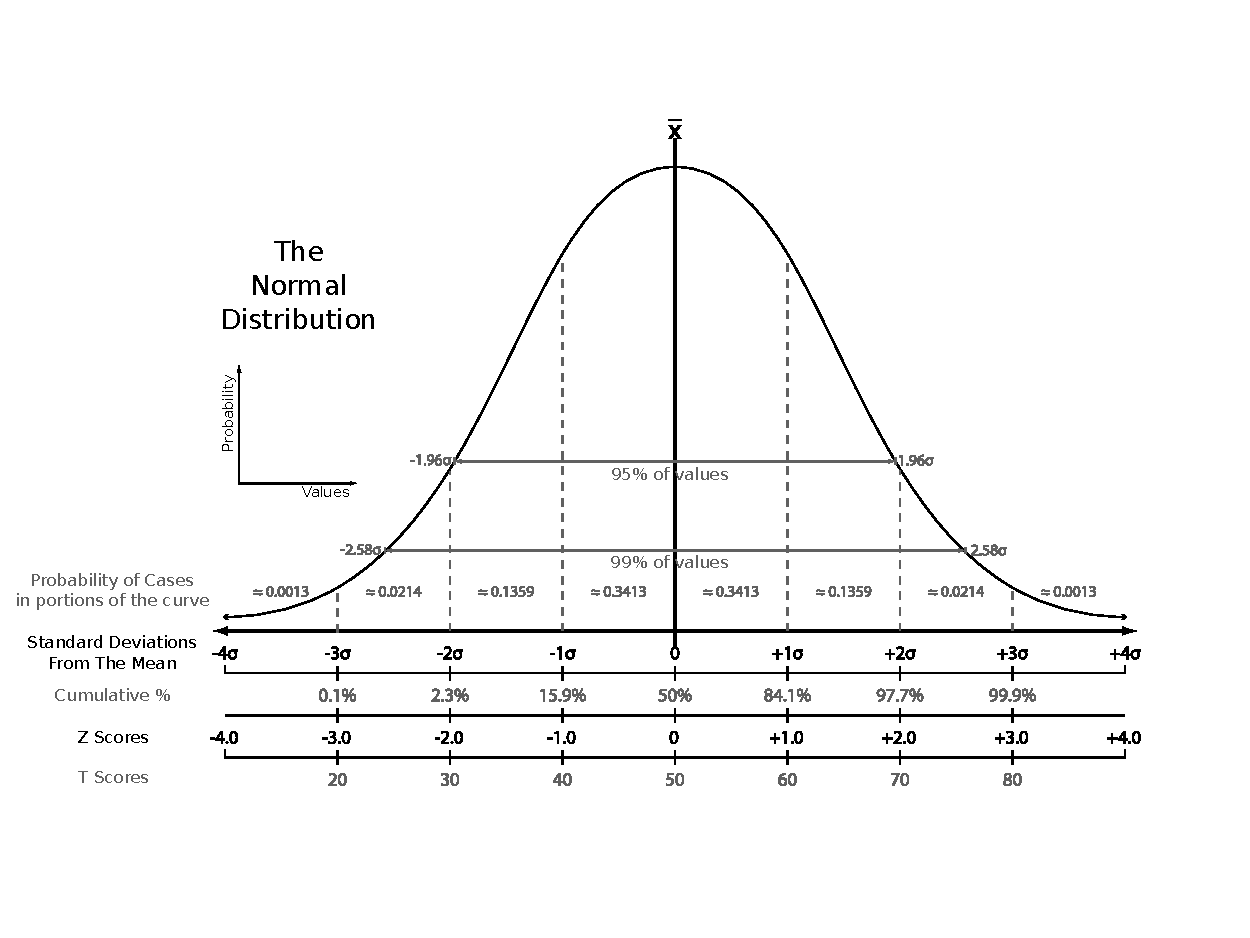
\includegraphics[width=0.8\textwidth]{The_Normal_Distribution.pdf}
	\caption{A~visualization of~the~concept of~standardized value for~a~normal distribution \cite{Wiki:z-score}}\label{fig:z-score}
\end{figure}
%
The mean for~the~U is~calculated by~the~formula
\begin{equation}\label{eq:U-mean}
m_{U} = \frac{n_{1}n_{2}}{2}.
\end{equation}
The~formula for~the standard deviation in~the case of~no~ties is~as~follows:
\begin{equation}\label{eq:standard-deviation-no-ties}
\sigma_{U} =  \sqrt{\frac{n_{1}n_{2}(n_{1}+n_{2}+1)}{12}}.
\end{equation}
In~case of~the~presence of~tied ranks, a~different formula is~used:
\begin{equation}\label{eq:standard-deviation-ties}
\sigma_{U_{ties}} = \sqrt{\frac{n_{1}n_{2}(n_{1}+n_{2}+1)}{12} - \frac{n_{1}n_{2}\sum_{k=1}^{K}({t_{k}}^{3} - t_{k})}{12n(n-1)}} = \sqrt{\frac{n_{1}n_{2}}{12} \left((n+1)-\frac{\sum_{k=1}^{K}({t_{k}}^{3} - t_{k})}{n(n-1)}\right)},
\end{equation}
where~$t_{k}$ is~the~number of~observations with rank~\textit{k} and \textit{K} is~the~total number of~tied ranks. Then, by~obtaining a~standardized value~(z-score) and~using an~approximation of~the~standard normal distribution, the~p-value for~a~given level of~significance (usually~0.05) is~calculated. The~interpretation of~the~result is~as~follows:
\begin{equation}\label{eq:p-interpretation}
\begin{aligned}
p &\leq 0.05 \Rightarrow \text{the~null hypothesis is~rejected}\\
p &> 0.05 \Rightarrow \text{the~null hypothesis can~not~be rejected}.
\end{aligned}
\end{equation}
However, there is~also an~alternative interpretation:
\begin{equation}\label{eq:p-interpretation-2}
\begin{aligned}
p &< 0.05 \Rightarrow \text{the~null hypothesis is~rejected}\\
p &\geq 0.05 \Rightarrow \text{the~null hypothesis can~not~be rejected}.
\end{aligned}
\end{equation}
To~date, there is~no~unambiguous position on~how the~situation when $p = \alpha$ should~be interpreted. This paper uses the~version described in~\ref{eq:p-interpretation}.
%
\section{Relationship to~other statistical tests}
\subsection{Comparison of~Wilcoxon-Mann-Whitney U-test with Student's t-test}
You often hear that the~U-test is~the~nonparametric counterpart of~the~Student's t-test, designed for~data whose distribution differs from the~normal one. From a~purely practical point of~view, we~can indeed say that in~the~case of~a~normal distribution it~is~advisable to~determine whether there is~a~significant difference between the~two samples by~means of~the~t-test, and in~the~case of~a~distribution that differs from the~normal by~means of~the~U-test. Thus, it~can~be said that these tests are~used for~the~same ultimate purpose.

However, the~mathematical meaning of~the~U-test and~the~t-test are~significantly different. As~stated earlier, the~U-test is~designed to~test the~null hypothesis, which is~that for~randomly chosen from two samples of~observations $x \in X$ and~$y \in Y$ the~probability that~\textit{x} is~greater than~\textit{y} is~equal to~the~probability that~\textit{y} is~greater than~\textit{x}, the~alternative hypothesis carries the~claim that these probabilities are~not equal. At~the~same time, the~t-test is~designed to~test the~null hypothesis that the~means of~the~two samples are~equal, while the~alternative hypothesis is~that the~means of~the~two samples are~not~equal. In~this regard, when comparing these tests, we~should keep in~mind that, in~general, the~U-test and~the~t-test check different null hypotheses, although they have partly similar practical meaning. The~result of~the~U-test is~most often very close to~the~result of~the~two-sample t-test for~ranked data. Table~\ref{tab:U-test-t-test-comparison} then provides a~general comparison of~the~U-test with the~t-test.
%
\begin{table}[ht]
	\caption{Properties of~the~U-test relative to~the~t-test.}  \label{tab:U-test-t-test-comparison}
	\centering
	\begin{tabularx}{\textwidth}{p{0.15\linewidth} p{0.8\linewidth}} 
		\hline
		Property&Description\\
		\hline
		Applicability to~ordinal data&When working with ordinal~(rank) data, rather than quantitative data, the~U-test is~preferable to~the~t-test, remembering that the~distance between neighboring values of~the~variation series cannot~be considered constant.\\
		\hline
		Robustness&Since the~U-test handles the~sum of~ranks rather than trait values, it~is less likely than the~t-test to~erroneously indicate significance due~to outliers. However, in~general, the~U-test is~more prone to~type~I error in~the~case when the~data simultaneously have the~property of~heteroscedasticity and~have a~distribution other than normal.\\
		\hline
		Efficiency&In~the~case of~a~normal distribution, the~asymptotic efficiency of~the~U-test is~$\frac{3}{4}\pi \approx 0.95$ of~the~t-test~\cite{U-test-efficiency}. If~the~distribution differs significantly from the~normal one and~the~number of~observations is~large enough, the~efficiency of~the~U-test is~significantly higher than the~efficiency of~the~t-test~\cite{Practical-Nonparametric-Statistics}. However, this efficiency comparison should~be interpreted with caution, because the~U-test and the~t-test examine different hypotheses and~estimate different values. In~the~case, for~example, of~the~need to~compare means, the~use of~the~U-test is~not justified in~principle.\\
		\hline
	\end{tabularx}
\end{table}
%
\subsection{Alternative tests in~the~case of~inequality of~distributions}
If~it~is necessary to~test the~stochastic ordering of~two samples (i.e.~the~alternative hypothesis: $H1:\ P(Y>X)+0.5P(Y=X)\neq0.5$) without assuming equality of~their distributions (i.e.~when the null hypothesis is~$H0:\ P(Y>X)+0.5P(Y=X)=0.5$ but not $F(X)=G(Y)$), more appropriate tests should~be used. These include the~Brunner-Munzel test~\cite{Bruner-Munzel-test-1}, which is~a~heteroskedasticity-resistant analog of~the~U-test, and the~Fligner-Policello test~\cite{Fligner-Policello-test}, which is~a~test for~equality of~medians. In~particular, in~the~case of~a~more general null hypothesis $H0:\ P(Y>X)+0.5P(Y=X)=0.5$, the~U-test can often lead to~a~type~I error even in~the case of~large samples (especially in~the~case of~disparity of~variance and significantly different sample sizes), so~that in~such cases the use of~alternative tests is~preferable~\cite{U-test-vs-Bruner-Munzel-test}. Thus, in~the absence of~the assumption of~equality of~distributions in~case the null hypothesis is~valid, the use of~alternative tests will~be preferable.

In~the case of~testing the hypothesis of~a~shift with significantly different distributions, the U-test may give an~erroneous interpretation of~significance~\cite{U-test-unequal-variance}, so~in~such circumstances it~is preferable to~use a~variant of~the \href{https://en.wikipedia.org/wiki/Welch's_t-test}{t-test}~\cite{Welch-t-test} designed for cases of~unequal variance~\cite{U-test-unequal-variance}. In~some cases, it~may~be justified to~convert quantitative data into ranks and then perform the t-test in~some variant depending on~the assumption of~equality of~variance. When converting quantitative data to~ordinal data, the original variances will not~be preserved; they must~be recalculated for the ranks themselves. In~the case of~equal variance, a~suitable nonparametric substitute for the \href{https://en.wikipedia.org/wiki/F-test}{F-test}~\cite{F-test} can~be the \href{https://en.wikipedia.org/wiki/Brown-Forsythe_test}{Brown-Forsythe test}~\cite{Brown-Forsythe-test}.
%
\subsection{The relationship between the U-test and the classification tasks}\label{U-test&classification}
The U-test is~a particular case of~the \href{https://en.wikipedia.org/wiki/Ordered_logit}{ordered logit model}~\cite{Ordered-logit}.
%
\section{The relationship between the U-test and the concepts of~Receiver operating characteristics~(ROC) and Area Under Curve~(AUC)}\label{U-AUC}
Based on~what was said in~\ref{U-test&classification}, we~can conclude that the U-test is~not only a~test for testing the shift hypothesis (or~another one similar in~meaning), but also represents a~kind of~classifier. Looking ahead, the meaning of~the U-test as~a~classifier is~as~follows:
\begin{itemize}
	\item there is~a~"positive" outcome of~comparing two random observations, which is~that the observation from~\textit{X} is~greater than the observation from~\textit{Y};
	\item the proportion of~the sum of~the ranks of~the "positive" elements is~calculated.
	\item as~in~general with ROC, if~the value of~the share of~"positive" elements exceeds~0.5, this means that the classifier generally performs its function; if~it~is equal to~0.5, its efficiency is~equal to~guessing with a~coin flip; if~it~is less than~0.5, using such classifier yields the opposite result.	 
\end{itemize}
At~first glance, the relationship between the U-test and ROC does~not seem obvious. This section will attempt to~understand why these concepts are related and what~is the essence of~the U-test as~a~classifier.

ROC analysis itself is~outside the scope of~this paper. Therefore, let~us consider only its main points.
\begin{description}
	\item[ROC curve ---] is~a~graphical plot that allows us to~evaluate the quality of~binary classification. It~displays the ratio between the proportion of~objects from the total number of~feature carriers correctly classified as~carrying the feature (True Positive Rate~(TPR), called the \emph{sensitivity of the classification algorithm}) and the proportion of~objects from the total number of~objects not carrying the feature, incorrectly classified as~carrying the feature (False Positive Rate~(FPR), the \textbf{1-FPR} value is~called the \emph{specificity of~the classification algorithm}), when varying the threshold of~the deciding rule.	It~is also known as~\textbf{error curve}. Analysis of~classifications using ROC curves is~called \textbf{ROC analysis}.
\end{description}
Quantitative interpretation of~the ROC curve gives the Area under curve~(AUC).
\begin{description}
	\item[Area under curve~(AUC) ---] is~the area bounded by~the ROC curve and the axis of~the proportion of~false positive classifications (abscissa axis).
\end{description}
The higher the AUC, the better the quality of~the classifier, while a~value of~0.5 demonstrates the unsuitability of~the chosen classification method (corresponding to~a~random coin guessing). A value of less than 0.5 indicates that the classifier works exactly the other way around: if you call positive results negative and vice versa, the classifier will perform better~\cite{Wiki:ROC}.

Let's introduce some terms.
\begin{description}
	\item[Condition positive~(P) --- ] the number of real positive cases in~the data.
	\item[Condition negative~(N)---] the number of real negative cases in the data.
	\item[True positive~(TP) ---] a~test result that correctly indicates the presence of~a~condition or~characteristic.
	\item[True negative~(TN) ---] a~test result that correctly indicates the absence of~a~condition or~characteristic.
	\item[False positive~(FP) ---] a~test result which wrongly indicates that a~particular condition or~attribute is~present.
	\item[False negative~(FN) ---] a~test result which wrongly indicates that a~particular condition or~attribute is~absent.
\end{description}
Based on~the above, we~can create a~contingency table of~the results of~applying the binary classifier. The rows contain data on~the actual presence or~absence of~the feature, the columns on~the predicted with the classifier.
%
\begin{table}[ht]
	\caption{Binary classifier contingency table.}  \label{tab:ROC-contingency-table}
	\centering
	\begin{tabularx}{\textwidth}{p{0.2\linewidth} p{0.375\linewidth} p{0.375\linewidth}} 
		\hline
	Total $P+N$&Predicted Positive~(PP)&Predicted negative~(PN)\\
		\hline
		Positive~(P)&TP&FN, type~II error~\cite{Wiki:type-1-2-errors}\\
		\hline
		Negative~(N)&FP, type~I error~\cite{Wiki:type-1-2-errors}&TN\\
		\hline
	\end{tabularx}
\end{table}
%
As~can~be seen from Table~\ref{tab:ROC-contingency-table}, the binary classifier can lead to~errors of~two types. Let's introduce some more definitions and define the formulas for calculating the probabilities of~its outcomes~(see tables~\ref{tab:ROC-rates-1}--\ref{tab:ROC-rates-3}).
%
\begin{table}[ht]
	\caption{Additional definitions and formulas for calculating the probabilities of binary classifier outcomes (part~1 of~3).}\label{tab:ROC-rates-1}
	\tiny
	\begin{tabularx}{\textwidth}{p{0.15\linewidth} p{0.4\linewidth} p{0.4\linewidth}} 
		\hline
		Notation&Formula&Deciphering the notation and alternative terms.\\
		\hline
		TPR~(SEN)&\begin{equation}\label{TPR}
		TPR=\frac{TP}{P}=1-FNR=\frac{TP}{TP+FN}
		\end{equation}&\href{https://en.wikipedia.org/wiki/Sensitivity_(test)}{\textbf{true positive rate}}, \href{https://en.wikipedia.org/wiki/Sensitivity_(test)}{\textbf{sensitivity}}~\cite{Wiki:sensitivity-and-specificity}, \href{https://en.wikipedia.org/wiki/Precision_and_recall}{recall}~\cite{Wiki:precision-and-recall}, probability of~detection, \href{https://en.wikipedia.org/wiki/Hit_rate}{hit rate}~\cite{Wiki:hit-rate}, power\\
		\hline
		FPR&\begin{equation}\label{eq:FPR}
		FPR = \frac{FP}{N} = 1 - TNR = \frac{FP}{FP+TN}
		\end{equation}&\href{https://en.wikipedia.org/wiki/False_positive_rate}{\textbf{false positive rate}}, probability of~false alarm, \href{https://en.wikipedia.org/wiki/False_positive_rate}{fall-out}~\cite{Wiki:FPR}\\
		\hline
		FNR&\begin{equation}\label{eq:FNR}
		FNR = \frac{FN}{P} = 1 - TPR = \frac{FN}{FN+TP}
		\end{equation}&\href{https://en.wikipedia.org/wiki/Type_I_and_type_II_errors\#False_positive_and_false_negative_rates}{\textbf{false negative rate}}~\cite{Wiki:TypeI-TypeII-errors}, miss rate\\
		\hline
		TNR~(SPC)&\begin{equation}\label{eq:TNR}
		TNR = \frac{TN}{N} = 1 - FPR = \frac{TN}{TN+FP}
		\end{equation}&\href{https://en.wikipedia.org/wiki/Sensitivity_(test)}{\textbf{true negative rate}}, \href{https://en.wikipedia.org/wiki/Sensitivity_(test)}{\textbf{specificity}}, \href{https://en.wikipedia.org/wiki/Sensitivity_(test)}{selectivity}~\cite{Wiki:sensitivity-and-specificity}\\
		\hline
		PPV&\begin{equation}\label{eq:PPV}
		PPV = \frac{TP}{TP+FP} = 1 - FDR
		\end{equation}&\href{https://en.wikipedia.org/wiki/Positive_and_negative_predictive_values}{\textbf{positive predictive value}}~\cite{Wiki:PPV}, \href{https://en.wikipedia.org/wiki/Information_retrieval\#Precision}{precision}~\cite{Wiki:precision}\\
		\hline
		NPV&\begin{equation}\label{eq:NPV}
		NPV = \frac{TN}{TN+FN} = 1 -FOR
		\end{equation}&\href{https://en.wikipedia.org/wiki/Positive_and_negative_predictive_values}{\textbf{negative predictive value}}~\cite{Wiki:PPV}\\
		\hline
		FDR&\begin{equation}\label{eq:FDR}
		FDR = \frac{FP}{FP + TP} = 1 - PPV
		\end{equation}&\href{https://en.wikipedia.org/wiki/False_discovery_rate}{\textbf{false discovery rate}}~\cite{Wiki:FDR}\\
		\hline
	\end{tabularx}
	\normalsize
\end{table}
%
\begin{table}[ht]
	\caption{Additional definitions and formulas for calculating the probabilities of binary classifier outcomes (part~2 of~3).}\label{tab:ROC-rates-2}
	\tiny
	\begin{tabularx}{\textwidth}{p{0.15\linewidth} p{0.4\linewidth} p{0.4\linewidth}} 
		\hline
		Notation&Formula&Deciphering the notation and alternative terms.\\
		\hline
		FOR&\begin{equation}\label{eq:FOR}
		FOR = \frac{FN}{FN+TN}=1-NPV
		\end{equation}&\href{https://en.wikipedia.org/wiki/Positive_and_negative_predictive_values}{\textbf{false omission rate}}~\cite{Wiki:PPV}\\
		\hline
		LR+&\begin{equation}\label{eq:LR+}
		LR+=\frac{TPR}{FPR}
		\end{equation}&\href{https://en.wikipedia.org/wiki/Likelihood_ratios_in_diagnostic_testing\#positive_likelihood_ratio}{\textbf{\textbf{positive likelihood ratio}}}~\cite{Wiki:likehoods-ratios}\\
		\hline
		LR-&\begin{equation}\label{eq:LR-}
		LR-=\frac{FNR}{TNR}
		\end{equation}&\href{https://en.wikipedia.org/wiki/Likelihood_ratios_in_diagnostic_testing\#negative_likelihood_ratio}{\textbf{negative likelihood ratio}}~\cite{Wiki:likehoods-ratios}\\
		\hline
		PT&\begin{equation}\label{eq:PT}
		PT=\frac{\sqrt{TPR(-TNR+1)}+TNR-1}{TPR+TNR-1}=\frac{\sqrt{FPR}}{\sqrt{TPR}+\sqrt{FPR}}
		\end{equation}&\href{https://en.wikipedia.org/wiki/Sensitivity_(test)}{\textbf{prevalence threshold}}~\cite{Wiki:sensitivity-and-specificity}\\
		TS~(CSI)&\begin{equation}\label{eq:TS|CSI}
		TS = \frac{TP}{TP+TN+FP}
		\end{equation}&\href{https://en.wikipedia.org/wiki/Jaccard_index\#Jaccard_index_in_binary_classification_confusion_matrices}{Jaccard index} \textbf{threat score}, \textbf{critical success index}~\cite{Wiki:jaccard-index}\\
		\hline
		PRV&\begin{equation}\label{eq:PRV}
		PRV = \frac{P}{P+N}
		\end{equation}&\href{https://en.wikipedia.org/wiki/Prevalence}{\textbf{prevalence}}~\cite{Wiki:prevalence}\\
		\hline
		ACC&\begin{equation}\label{eq:ACC}
		ACC = \frac{TP+TN}{P+N} = \frac{TP+TN}{TP+TN+FP+FN}
		\end{equation}&\href{https://en.wikipedia.org/wiki/Accuracy_and_precision}{\textbf{accuracy}}~\cite{Wiki:accuracy-precision}\\
		\hline
	\end{tabularx}
	\normalsize
\end{table}
%
\begin{table}[ht]
	\caption{Additional definitions and formulas for calculating the probabilities of binary classifier outcomes (part~3 of~3).}\label{tab:ROC-rates-3}
	\tiny
	\begin{tabularx}{\textwidth}{p{0.15\linewidth} p{0.4\linewidth} p{0.4\linewidth}} 
		\hline
		Notation&Formula&Deciphering the notation and alternative terms.\\
		\hline
		BA&\begin{equation}\label{eq:BA}
		BA = \frac{TPR+TNR}{2}
		\end{equation}&\textbf{balanced accuracy}\\
		\hline
		F1 score&\begin{equation}\label{eq:F1-score}
		F_{1} = 2 \times \frac{PPV \times TPR}{PPV +TPR} = \frac{2TP}{2TP + FP + FN}
		\end{equation}&\href{https://en.wikipedia.org/wiki/F-score}{F1 score} is~the harmonic mean of~\href{https://en.wikipedia.org/wiki/Information_retrieval\#Precision}{precision} and \href{https://en.wikipedia.org/wiki/Sensitivity_(test)}{sensitivity}~\cite{Wiki:F-score}\\
		\hline
		MCC~($\phi$ or~$r_{\phi}$)&\begin{equation}\label{eq:MCC}
		MCC = \frac{TP \times TN - FP \times FN}{\sqrt{(TP+FP)(TP+FN)(TN+FP)(TN+FN)}}
		\end{equation}&\href{https://en.wikipedia.org/wiki/Phi_coefficient}{\textbf{Matthews correlation coefficient}},\href{https://en.wikipedia.org/wiki/Phi_coefficient}{\textbf{phi coefficient}}~\cite{Wiki:phi-coefficient}\\
		\hline
		FM&\begin{equation}\label{eq:FM}
		FM = \sqrt{\dfrac{TP}{TP+FP} \times \dfrac{TP}{TP+FN}} = \sqrt{PPV \times TPR}
		\end{equation}&\href{https://en.wikipedia.org/wiki/Fowlkes–Mallows_index}{Fowlkes–Mallows index}~\cite{Wiki:Fowlkes–Mallows-index}\\
		\hline
		BM&\begin{equation}\label{eq:BM}
		BM = TPR + TNR -1
		\end{equation}&\textbf{bookmaker informedness}, \href{https://en.wikipedia.org/wiki/Youden's_J_statistic}{informedness}~\cite{Wiki:j-statistic}\\
		\hline
		MK~($\delta P$)&\begin{equation}\label{eq:MK}
		MK = PPV + NPV - 1
		\end{equation}&\href{https://en.wikipedia.org/wiki/Markedness}{\textbf{markedness}}, deltaP~\cite{Wiki:markedness}\\
		\hline
		DOR&\begin{equation}\label{eq:DOR}
		\frac{LR+}{LR-}
		\end{equation}&\href{https://en.wikipedia.org/wiki/Diagnostic_odds_ratio}{\textbf{diagnostic odds ration}}~\cite{Wiki:DOR}\\
		\hline
	\end{tabularx}
	\normalsize
\end{table}
%
The TPR probability can~be written as
\begin{equation}\label{eq:TPR-probability}
P_{TPR} = \mathbb{P}(1,\ x\in C_{1}),
\end{equation}
which means that if~object~\textit{x} belongs to~class~$C_{1}$, this indicator estimates the probability that the binary classifier assigns object~\textit{x} to~this class. The probability of~FPR is~written as
\begin{equation}\label{eq:FPR-probability}
P_{FPR} = \mathbb{P}(1,\ x\in C_{0}),
\end{equation}
which means the probability that an~object belonging to class~$C_0$ will~be mistakenly assigned to~class~$C_1$.

Typically, the working principle of~a~binary classifier is~based on~comparing the measurement of~\textit{x} with some fixed threshold~\textit{c}. It~follows that the previous two expressions can~be rewritten and combined into a~system.
\begin{equation}\label{eq:TRP+FPR-probability}
\begin{cases}
P_{TPR} = \mathbb{P}(x>c,\ x \in C_{1})\\
P_{FPR} = \mathbb{P}(x>c,\ x \in C_{0})
\end{cases}
\end{equation}
It~follows that the ROC curve is~a~diagram
\begin{equation}\label{eq:ROC-contour}
P_{FPR}(c),\ P_{TPR}(c),
\end{equation}
thus, drawing the curve means changing the value of~threshold~\textit{c}.

Let's consider the example~\cite{AUC-Derivation}. Let's take~$f(x\in C_{0}) = \mathcal{N}(0,1)$ and~$f(x\in C_{1}) = \mathcal{N}(2,1)$ as~probability density functions~$C_{0}$ and~$C_{1}$, respectively. Next we~build the ROC curve step by~step using the Python language. At~the first step, consider diagram~\ref{fig:plot-TPR-FPR-prob-density-1}, built using the code given in~script~\ref{lst:plot-TPR-FPR-prob-density}. The area shaded blue shows the probability of~FPR, i.\,e., false-positive significance detection, while the area shaded green shows the probability density of TPR, i.\,e., correct significance detection. The ROC curve shows the values of~these very indicators. The vertical dashed line is~the sensitivity threshold~\textit{c}. In~this situation it~is at~0 on~the abscissa axis. If~it~is moved to~1, the area under the FPR curve (blue) will significantly decrease, i.\,e. the probability of~false-positive detection will decrease, but the TPR area (green) will decrease as~well, which means an~increase in~the probability of~false-negative results. This situation is~illustrated in~Diagram~\ref{fig:plot-TPR-FPR-prob-density-2}.
%
\begin{figure}[ht]
	\centering
	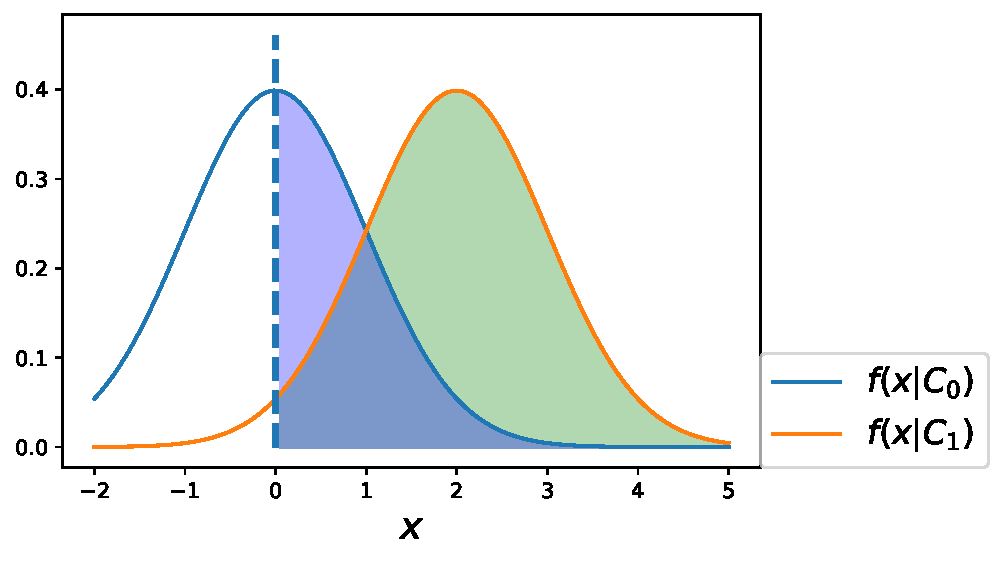
\includegraphics[width=0.95\textwidth]{Plot-ROC-step-1.pdf}
	\caption{Diagram of~TPR and FPR probability distribution densities at~threshold~0.}
	\label{fig:plot-TPR-FPR-prob-density-1}
\end{figure}
%
\begin{lstlisting}[float, caption = Plotting TPR and FPR probability density functions, firstnumber=1, label= lst:plot-TPR-FPR-prob-density]
# Import Libraries
import numpy as np
import matplotlib.pyplot as plt
from scipy import stats

# Plot
f0 = stats.norm(0, 1)
f1 = stats.norm(2, 1)
fig, ax = plt.subplots()
xi = np.linspace(-2, 5, 100)
ax.plot(xi, f0.pdf(xi), label=r'$f(x|C_0)$')
ax.plot(xi, f1.pdf(xi), label=r'$f(x|C_1)$')
ax.legend(fontsize=16, loc=(1, 0))
ax.set_xlabel(r'$x$', fontsize=18)
ax.vlines(0, 0, ax.axis()[-1] * 1.1, linestyles='--', lw=3.)
ax.fill_between(xi, f1.pdf(xi), where=xi > 0, alpha=.3, color='g')
ax.fill_between(xi, f0.pdf(xi), where=xi > 0, alpha=.3, color='b')

# Save to .pdf
plt.savefig('Plot-ROC-step-1.pdf', bbox_inches='tight')

\end{lstlisting}
%
\begin{figure}[ht]
	\centering
	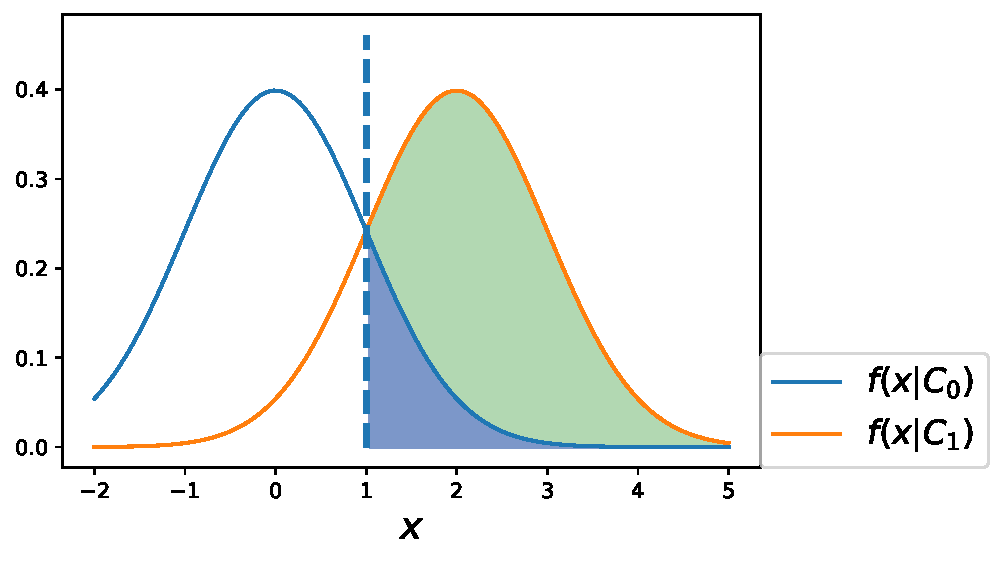
\includegraphics[width=0.95\textwidth]{Plot-ROC-step-2.pdf}
	\caption{Diagram of~TPR and FPR probability distribution densities at~threshold~1.}
	\label{fig:plot-TPR-FPR-prob-density-2}
\end{figure}

As~you can see from the diagrams above, increasing the threshold leads to~the loss of~a~part of~both true-positive and false-positive results, while decreasing~it leads to~an~increase in~the number of~fixations of~the feature presence (both true and false). In~extreme cases, too low a~threshold value will lead to~the fact that all results will~be interpreted as~positive, too high --- to~a~zero number of~observations in~which the feature was detected. The task of~ROC analysis is~to~choose a~rational threshold value.

Let's add the ROC curves corresponding to~thresholds~0 and~1 to~the already existing diagrams. And also create an~interactive diagram using the code from script~\ref{lst:plot-TPR-FPR-prob-density+ROC-interactive}. The PDF format does~not allow you to~add such interactive elements, so~let's consider cases with fixed values of~0 and~1, shown in~Diagrams~\ref{fig:plot-TPR-FPR-prob-density-3} and \ref{fig:plot-TPR-FPR-prob-density-4}, respectively. The left side of~each of~them shows the already familiar probability density function graphs for the TPR and FPR distributions. The right part shows the ROC curve and the point corresponding to~the set threshold value. It~is easy to~guess that the x-coordinate of~the point matches the area under the FPR curve, and the y-coordinate matches the area under the TPR curve. Increasing the threshold value entails shifting the point to~the left, decreasing~it to~the right.

The better the binary classifier itself, the closer to~the upper left corner will~be the ROC curve corresponding to~it, because in~this case a~high TPR value will~be combined with a~low FPR value. The binary classifier, which works as~well (actually badly) as~the coin flip guessing algorithm (in~case the coin is~"fair"), gives a~ROC curve, which is~a~straight line between~(0,0) and~(1,1). In~this case, the left part of~the diagram will show a~complete overlap of~TPR and FPR probability density function curves. Such a~case is~shown in~Diagram~\ref{fig:plot-TPR-FPR-prob-density-3}. For self-practice, you can use Script~\ref{lst:plot-TPR-FPR-prob-density+ROC-interactive} by~running~it in~the Jupyter Lab environment, which allows you to~use the interactive features of~the browser.
%
\begin{lstlisting}[float, caption = Build an~interactive graph of~TPR and FPR distribution density and its corresponding ROC curve for a~given threshold value, firstnumber=1, label= lst:plot-TPR-FPR-prob-density+ROC-interactive]
# Import Libraries
%matplotlib inline
from ipywidgets import interact
import numpy as np
import matplotlib.pyplot as plt
from scipy import stats

# Plot
f0 = stats.norm(0, 1)
f1 = stats.norm(2, 1)
fig, ax = plt.subplots()
xi = np.linspace(-2, 5, 100)
ax.plot(xi, f0.pdf(xi), label=r'$f(x|C_0)$')
ax.plot(xi, f1.pdf(xi), label=r'$f(x|C_1)$')
ax.legend(fontsize=16, loc=(1, 0))
ax.set_xlabel(r'$x$', fontsize=18)
ax.vlines(0, 0, ax.axis()[-1] * 1.1, linestyles='--', lw=3.)
ax.fill_between(xi, f1.pdf(xi), where=xi > 0, alpha=.3, color='g')
ax.fill_between(xi, f0.pdf(xi), where=xi > 0, alpha=.3, color='b')

# Plot ROC-curve and make all interactive
def plot_roc_interact(c=0):
xi = np.linspace(-3,5,100)
fig,axs = plt.subplots(1,2)
fig.set_size_inches((10,3))
ax = axs[0]
ax.plot(xi,f0.pdf(xi),label=r'$f(x|C_0)$')
ax.plot(xi,f1.pdf(xi),label=r'$f(x|C_1)$')
ax.set_xlabel(r'$x$',fontsize=18)
ax.vlines(c,0,ax.axis()[-1]*1.1,linestyles='--',lw=3.)
ax.fill_between(xi,f1.pdf(xi),where=xi>c,alpha=.3,color='g')
ax.fill_between(xi,f0.pdf(xi),where=xi>c,alpha=.3,color='b')
ax.axis(xmin=-3,xmax=5)
crange = np.linspace(-3,5,50)
ax=axs[1]
ax.plot(1-f0.cdf(crange),1-f1.cdf(crange))
ax.plot(1-f0.cdf(c),1-f1.cdf(c),'o',ms=15.)
ax.set_xlabel('False-alarm probability')
ax.set_ylabel('Detection probability')

interact(plot_roc_interact,c=(-3,5,.05))

\end{lstlisting}
%
\begin{figure}[ht]
	\centering
	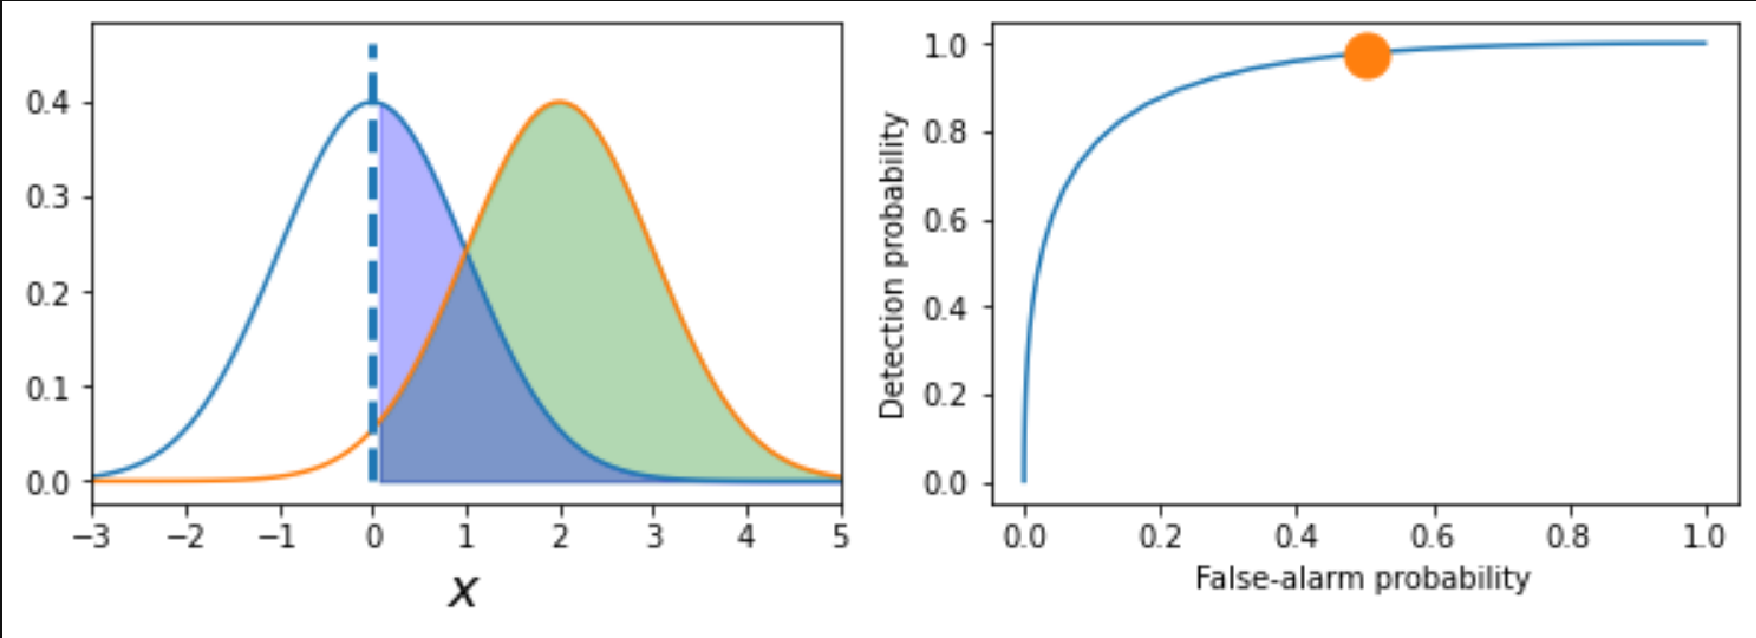
\includegraphics[width=0.95\textwidth]{Plot-ROC-step-30.pdf}
	\caption{Diagram of~TPR and FPR probability distribution densities at~threshold~0.}
	\label{fig:plot-TPR-FPR-prob-density-3}
\end{figure}
%
\begin{figure}[ht]
	\centering
	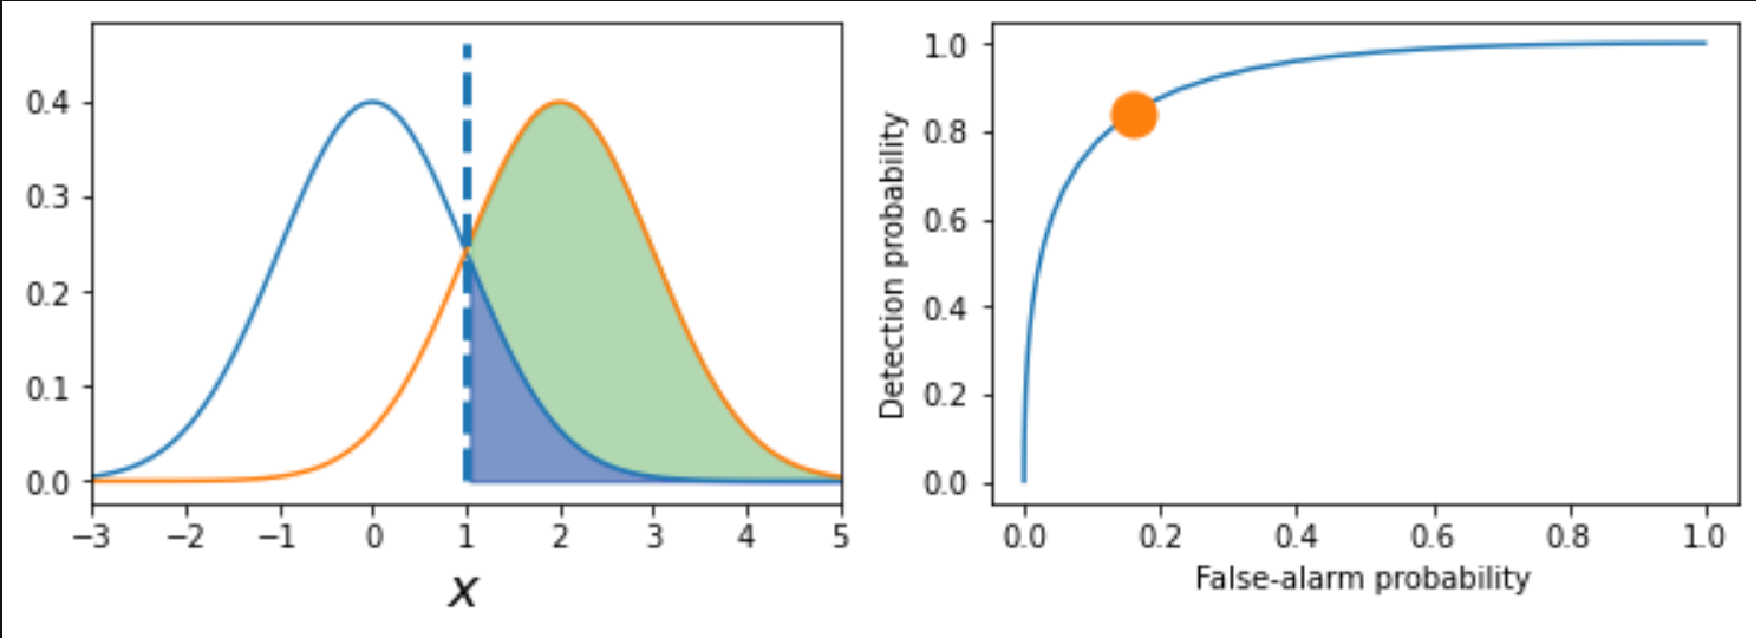
\includegraphics[width=0.95\textwidth]{Plot-ROC-step-4.pdf}
	\caption{Diagram of TPR and FPR probability distribution densities at threshold 1.}
	\label{fig:plot-TPR-FPR-prob-density-4}
\end{figure}
%
\begin{figure}[ht]
	\centering
	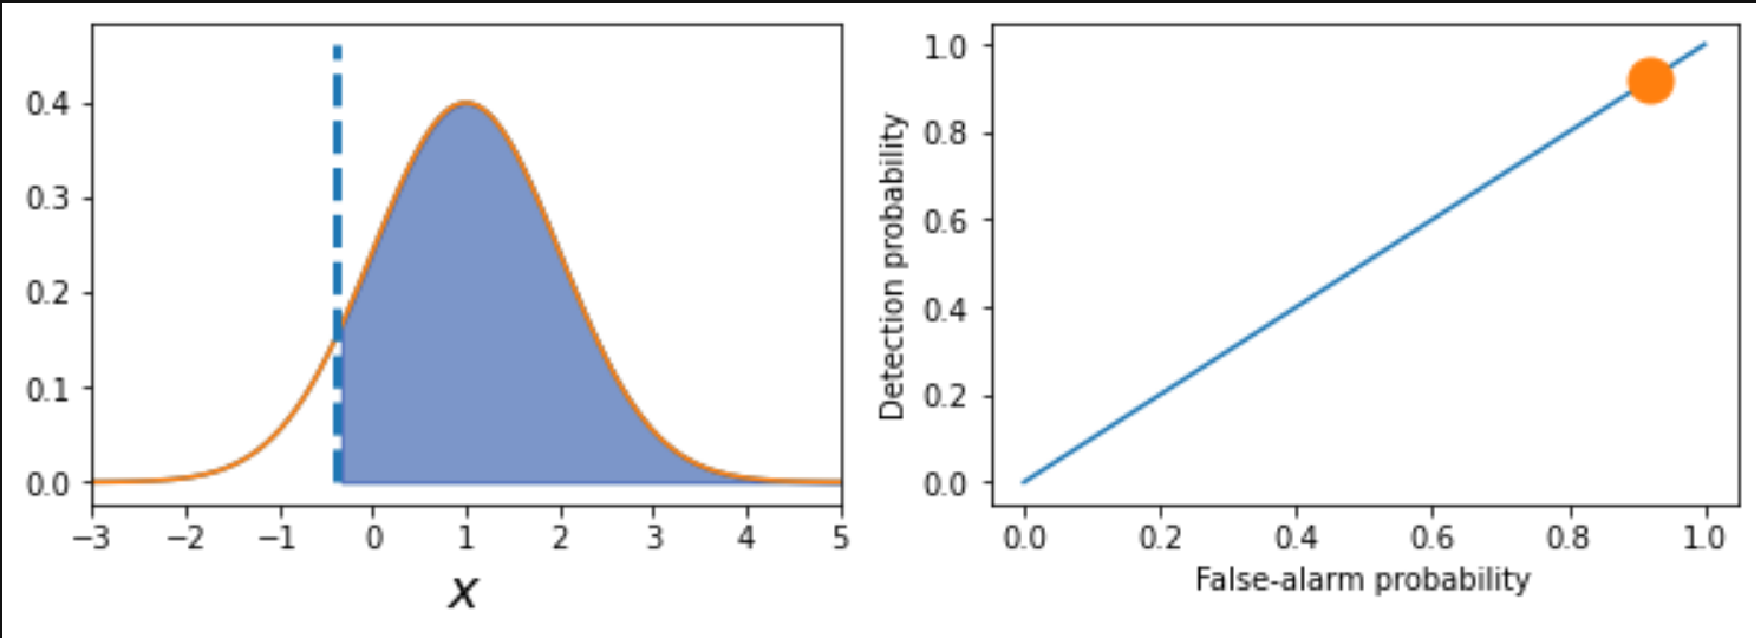
\includegraphics[width=0.95\textwidth]{Plot-ROC-step-5.pdf}
	\caption{Diagram of~probability densities of~TPR and FPR probability distributions at~equal mean.}
	\label{fig:plot-TPR-FPR-prob-density-5}
\end{figure}
%
\subsection{The concept of~AUC and its calculation}
As~the name implies, the AUC is~the area under the ROC curve bounded by~the point corresponding to~a~given threshold value. In~the normalized space in~which the ROC curve is~usually plotted, the AUC value is~equivalent to~the probability that the classifier assigns a~higher weight to~a~randomly chosen positive entity than to~a~randomly chosen negative entity. The AUC does not depend on~a~specific threshold value, because the ROC curve is~constructed by~fitting~it. This means that the AUC is~calculated by~integrating over the thresholds. The AUC is~given by~the expression:
\begin{equation}\label{eq:AUC-computation-0}
AUC = \int P_{TPR}(P_{FPR}) d P_{FPR}.
\end{equation}
The step-by-step calculation of~the AUC is~as~follows.
\begin{equation}\label{eq:AUC-computation-1}
P_{TPR}(c) = 1 - F_{1}(c),
\end{equation}
where~$F_{1}$ is~the cumulative density function for~$C_{1}$. Similarly calculate
\begin{equation}\label{eq:AUC-computation-2}
P_{FPR}(c) = 1 - F_{0}(c),
\end{equation}
where~$F_{0}$ is~the cumulative density function for~$C_{0}$.


Let~us take some particular value of~$c^{*}$ to~which a~certain~$P_{FPR}(c^{*})$ corresponds. In~other words, it~corresponds to~the probability that a~random element~$x_{0}$ belonging to~class~$C_{0}$ is~greater than the threshold value~$c^{*}$, i.e.
\begin{equation}\label{eq:AUC-computation-3}
P_{FPR}(c^{*}) = \mathbb{P}(x_{0}>c^{*}|x_{0} \in C_{0}).
\end{equation}
Then, reasoning similarly with respect to~TPR, we~get
\begin{equation}\label{eq:AUC-computation-4}
P_{TPR}(c^{*}) = \mathbb{P}(x_{1}>c^{*}|x_{1} \in C_{1}).
\end{equation}
Next, based on~the fact that the AUC is~realized through an~integral, we~select its value so~that the distribution of~$c^{*}$ matches the distribution of~$F_{0}$. In~this case,~$P_{TPR}$ is~an~independent random variable with a~corresponding expectation in~the form of
\begin{equation}\label{eq:AUC-computation-integral}
\mathbb{E}(P_{TPR}) = \int P_{TPR} d P_{FPR} = AUC.
\end{equation}
It~is~now possible to~formulate a~definition for the AUC.
\begin{description}
	\item[AUC ---] is~the expected probability that element~$x_{1} \in C_{1}$ will~be assigned to~$C_{1}$ with higher probability than element~$x_{0} \in C_{0}$. Thus,
	\begin{equation}\label{eq:AUC-definition}
	1-F_{1}(t)>1-F_{0}(t) \forall t.
	\end{equation}
	The wording "for any t" means that~$1-F_{1}(t)$ is~\emph{stochastically} greater than~$1-F_{0}(t)$. The latter circumstance is~key in~terms of~the relationship of~the AUC to~the U-test, which will~be shown later.
\end{description}
%
\subsection{Relation between U-test and AUC}\label{U-test&AUC-relation}
A~fairly detailed description of~the U-test was given earlier. This subsection contains only brief information about~it, which is~directly relevant to~the question of~its relationship to~the AUC.

The U-test is~a~non-parametric test that allows you to~test whether two samples belong to~the same distribution. His basic idea is~that if~there is~no~difference between two classes, then combining them into one larger class (set) and then calculating any statistic for the new larger class will give an~unbiased estimate for any of~the initial classes. In~other words, if~there is~no~difference in~the distribution of~the two samples, combining them and assuming that the actually observed data from the two samples represent only one of~the equal-valued variants of~the moving observations means that there is~no~difference in~any statistical estimate for any of~the moving variants relative to~the other, and relative to~the combined set.

Let's suppose that we~need to~compare two samples using the median, the mean, or~some other measure of~central tendency. In~terms of~cumulative distribution functions for the two populations, in~the case of~$H0$ we~have the following:
\begin{equation}\label{eq:U-AUC-H0}
H_0: F_{X}(t) = F_{Y}(t), \quad \forall t,
\end{equation}
which indicates that all observations belong to~the same distribution. Then an~alternative hypothesis is~that
\begin{equation}\label{eq:U-AUC-H1}
H_1: F_{X}(t) < F_{Y}(t), \quad \forall t,
\end{equation}
which is~possible, in~particular, in~the case of~the existence of~a~shift of~one distribution relative to~the other. In~this case, the samples ${X_{i}}_{i=1}^{n},\ {X_{j}}_{j=1}^{m}$ represent independent groups of~observations. In~this case, the size of~the samples may vary.

The test technique consists of~combining two samples into one set and assigning ranks to~each item within~it. The U-statistic is~the sum of~the ranks for the set~\textit{X}. If~the value of~the statistic is~small enough, it~means that the distribution of~set~\textit{X} is~stochastically shifted to~the left relative to~the distribution of~set~\textit{Y}, i.\,e.~$F_{X}{t} < F_{Y}{t}$.

Since with a~sufficiently large number of~observations (20 or~more) the distribution of~U-statistics is~well approximated by~the normal distribution, the p-value is~suitable for assessing significance. Let's calculate it~using the Python language according to~the script~\ref{lst:AUC-p-value}.
%
\begin{lstlisting}[float, caption = Calculation of~the p-value for the test data, firstnumber=1, label= lst:AUC-p-value]
print('p-value:',stats.wilcoxon(f1.rvs(30), f0.rvs(30))[1])

\end{lstlisting}
The p-value is~1.9729484515803686e-05, which is~less than the significance level~(0.05), so~we~can reject the null hypothesis~\ref{eq:U-AUC-H0}. Since the data were randomly generated, if~the experiment is~repeated, the particular p-value will differ from that obtained when writing this paper. However, it~will always be below the threshold because of~the parameters set in~the algorithm.

The U-statistic can be~written as~follows:
\begin{equation}\label{eq:U-statistics}
U = \frac{1}{mn}\sum_{i=1}^{m}\sum_{j=1}^{n}\mathbbm{1}{(Y_{j}>X_{i})},
\end{equation}
where~$\mathbbm{1}{(Y_{j}>X_{i})}$ is~the indicator (characteristic) function showing that the statistic (for the discrete case) estimates the probability that~\textit{Y} is~stochastically greater than~\textit{X}. Thus, this correspondence means that its value is~equal to~the AUC. The relationship between the AUC and the U-test is~in a~similar sense: checking the stochastic excess value of~observations belonging to~one sample relative to~observations belonging to~another sample.
%
\subsection{Practice of~ROC analysis and AUC calculation.}\label{ROC-AUC-theory}
This subsection is~not required reading if~the goal is~only the practical implementation of~the U-test itself. However, it~gives an~insight into machine learning methods that are not related to~the so-called \emph{frequentist statistics} to~which the U-test itself belongs, and shows the relationship between these areas of~data analysis. In~addition, it~will provide sufficient knowledge to~perform a~ROC analysis as~such, which may~be useful in~other situations that an~appraiser may encounter in~his or~her practice.
%
\subsubsection{Plotting the ROC curve}\label{plot-ROC-theory}
%
\lstset{language=R,
	basicstyle=\ttfamily,
	keywordstyle=\color{Blue}\ttfamily,
	stringstyle=\color{Red}\ttfamily,
	commentstyle=\color{Emerald}\ttfamily,
	morecomment=[l][\color{Magenta}]{\#},
	breaklines=true,
	breakindent=0pt,
	breakatwhitespace,
	columns=fullflexible,
	showstringspaces=false
}
%
ROC analysis and in~particular the construction of~ROC curves are widely used to~find a~compromise between the \emph{sensitivity} and \emph{specificity} of~a~binary classifier. Most of~the classifiers used in~machine learning produce a~result in~the form of~a~quantification that a~given object has a~"positive" feature value. Some threshold value is~needed to~convert such a~quantitative assessment into a~concrete "yes" or~"no" prediction. In~his case, observations with a~score above this threshold will~be classified as~"positive", below as~"negative". Different thresholds provide different levels of~sensitivity and specificity. Setting a~relatively high threshold value provides a~conservative approach to~the issue of~classifying a~particular case as "positive", which reduces the likelihood of~false positives. At~the same time, this increases the risk of~missing the observed positive values, i.\,e., it~reduces the level of~true positive classification results. A~relatively low threshold value provides a~more liberal approach to~classifying observations as~"positive".  This reduces specificity (increases the number of~false negatives) and increases sensitivity (increases the number of~true positives). The ROC curve shows the ratio of~true positives to~false positives, giving an~overview of~the entire spectrum of~such trade-offs. There are many R~language libraries that plot ROC curves and calculate metrics for ROC analysis. In~this case, to~better understand the essence of~ROC analysis, some actions will~be performed by~writing our own functions. The following will show an~algorithm for constructing a~ROC curve based on~a~set of~real outcomes and their corresponding estimates. The calculation involves two steps:
\begin{itemize}
	\item sort the observed outcomes in~descending order by~their predicted scores;
	\item calculation of~total true positive (TPR) and true negative (TNR) scores for ordered observed outcomes.
\end{itemize}
Let's create an appropriate function (script~\ref{lst:create-ROC-function-R}).
%
\begin{lstlisting}[float, caption = Creating a~function to~calculate TPR and FPR, firstnumber=1, label= lst:create-ROC-function-R]
# create own function for ROC
appraiserRoc <- function(labels, scores){
labels <- labels[order(scores, decreasing=TRUE)]
data.frame(TPR=cumsum(labels)/sum(labels),
FPR=cumsum(!labels)/sum(!labels), labels)
}
 
\end{lstlisting}
%
This function has two inputs:
\begin{itemize}
	\item \emph{labels} --- Boolean vector containing actual classification data;
	\item \emph{scores} --- a~vector of~real numbers containing data about the scores predicted by~some classifier.
\end{itemize}
%
Since only two classification outcomes are possible, the labels vector can only contain \emph{TRUE} or~\emph{FALSE} values (or~\emph{1} and~\emph{0} depending on~the analyst's preference). A~sequence of~such binary values can~be interpreted as~a~set of~instructions for a~\href{https://en.wikipedia.org/wiki/Turtle_graphics}{turtle graphics}~\cite{Wiki:turtle-graphics}. There~is one important feature: in~this case the turtle has a~compass and receives instructions for absolute directions of~movement: "to~the north" or~"to~the east" instead of~relative "to~the right" and "to~the left". The turtle starts its movement from the starting point with coordinates~(0,0) and makes its way on~the plane according to~the sequence of~instructions. When a~\emph{TRUE} command is~received, it~takes one step north, i.\,e., in~the positive direction of~the y-axis, and when a~\emph{FALSE} command is~received, it~takes one step east, i.\,e., in~the positive direction of~the x-axis. The length of~the steps is~chosen in~such a~way that if~all \emph{TRUE~(1)} commands are received consecutively, the turtle will~be at~a~point with coordinates~(0,1), all \emph{FALSE~(0)} commands at~a~point with coordinates~(1,0). Thus, the length of~the step "to~the north" may~be different from the length of~the step "to~the east". The path in~the plane is~determined by~the order of~the \emph{TRUE~(1)} and \emph{FALSE~(0)} commands and always ends at~(1,1).

Advancing the turtle through the bits of~the instruction string is~an~adjustment of~the classification threshold to~less and less stringent. Once the turtle has passed the bit, it~means that it~has decided to~classify that bit as~"positive". If~this bit was actually "positive", it~is a~true positive, if~it~was actually "negative" it~is a~false positive. The y-axis shows the TPR, calculated as~the ratio of~the number of~positive results detected to~this time to~the total number of~actual positive results. The x-axis shows the (FPR), calculated as~the ratio of~the number of~currently detected positive results to~the total number of~actual negative results. The vectorized implementation of~this logic uses cumulative sums (the \textbf{cumsum} function) instead of~going through the values one by~one, although that is~what the computer does at~a~lower level.

The ROC curve calculated in~this way is~actually a~step function. With a~very large number of~positive and negative cases, these steps are very small, and the curve looks smooth. In~this case, with a~really large number of~observations, the construction of~each point is~difficult. As~a~consequence, in~practice, most ROC curve functions used for practical purposes contain additional steps and often use some form of~approximation.

As~an~example, consider a~situation in~which an~appraiser evaluates parts manufactured by~an~enterprise. Some of~the parts are known to~be of~good quality and some are defective. The valuation of~quality parts is~carried out on~the basis of~cost market approaches in~the usual manner. And defective parts are valued at~a~scrap value. In~this case, it~is necessary to~assign each part to~one or~another category. There is~some feature~\emph{x}, which can~be measured by~the appraiser. And there is~also some feature~\emph{y}, which cannot~be measured by~the appraiser. The value of~the feature~\emph{y} allows you to~classify parts as~quality or~defective. It~is also known that there is~some finitary relation function between features \emph{x} and~\emph{y}. Thus, knowing the value of~\emph{x}, we~can infer the value of~y with some probability.
In~this case, it~is advisable to~take a~certain sample of~parts. Then, together with the specialists of~the customer company, measure the values of~features \emph{0} and~\emph{y} for each element of~this sample.

We~will use simulated data to~consider the example. There is~some input feature~\emph{x} that is~linearly related to~the implicit result~\emph{y}. This relationship implies the presence of~some randomness. The y-value shows whether the part exceeds the tolerance requirements. If~so, it~should~be classified as~defective. The algorithm used in~this paper involves the following steps:
\begin{itemize}
	\item create the~\textbf{sim\_parts\_data} function that generates data according to~certain rules and sets the $"y>100"$ threshold value to~classify parts as~defective.
	\item create the~dataframe \textbf{parts\_data} with this function;
	\item create the~\textbf{test\_set\_idx} rule, whereby 80\,\% of~the data is~randomly assigned to~the training sample, and 20\,\% to the test sample;
	\item applying the rule \textbf{test\_set\_idx} to~data \textbf{parts\_data};
	\item create training (\textbf{<<training\_set>>}) and testing (\textbf{<<test\_set>>}) sub-samples;
	\item plot the diagram showing the distribution of~observations from the training sample.
\end{itemize}
To~implement the above algorithm, the code from script~\ref{lst:create-sample-data-plot-graph-R} was used.
%
\begin{lstlisting}[float, caption = Creation and primary visualization of~data on~quality and defective parts, firstnumber=1, label= lst:create-sample-data-plot-graph-R]
# Sample of ROC-analysis

# enable libraries
library(ggplot2)
library(dplyr)
library(pROC)

#set seed
set.seed(19190709)

# create own function for ROC
appraiserRoc <- function(labels, scores){
labels <- labels[order(scores, decreasing=TRUE)]
data.frame(TPR=cumsum(labels)/sum(labels),
FPR=cumsum(!labels)/sum(!labels), labels)
}

# create function 
sim_parts_data <- function(N, noise=100){
x <- runif(N, min=0, max=100)
y <- 122 - x/2 + rnorm(N, sd=noise)
bad_parts <- factor(y > 100)
data.frame(x, y, bad_parts)
}

# create dataset
parts_data <- sim_parts_data(2000, 10)

# create rule for test subset
test_set_idx <- sample(1:nrow(parts_data), size=floor(nrow(parts_data)/4))

# create training and test subsets
test_set <- parts_data[test_set_idx,]
training_set <- parts_data[-test_set_idx,]

# plot graph
test_set %>% 
ggplot(aes(x=x, y=y, col=bad_parts)) + 
scale_color_manual(values=c("green", "red")) + 
geom_point() + 
ggtitle("Bad parts related to x")

\end{lstlisting}
%

The result was diagram~\ref{fig:bad-parts-r}. As~you can see, if~the value of~the parameter~\emph{x} is~less than~15, all dots are red, which means that the parts are defective. Above 96 ерун are green, which means that the parts are of good quality. If~the value is~higher than 96, they are green, which means that the parts are of good quality. Between these values is~an area of~uncertainty, the right side of~which is~dominated by~green dots, and the left side by~red dots.
%
\begin{figure}[ht]
	\centering
	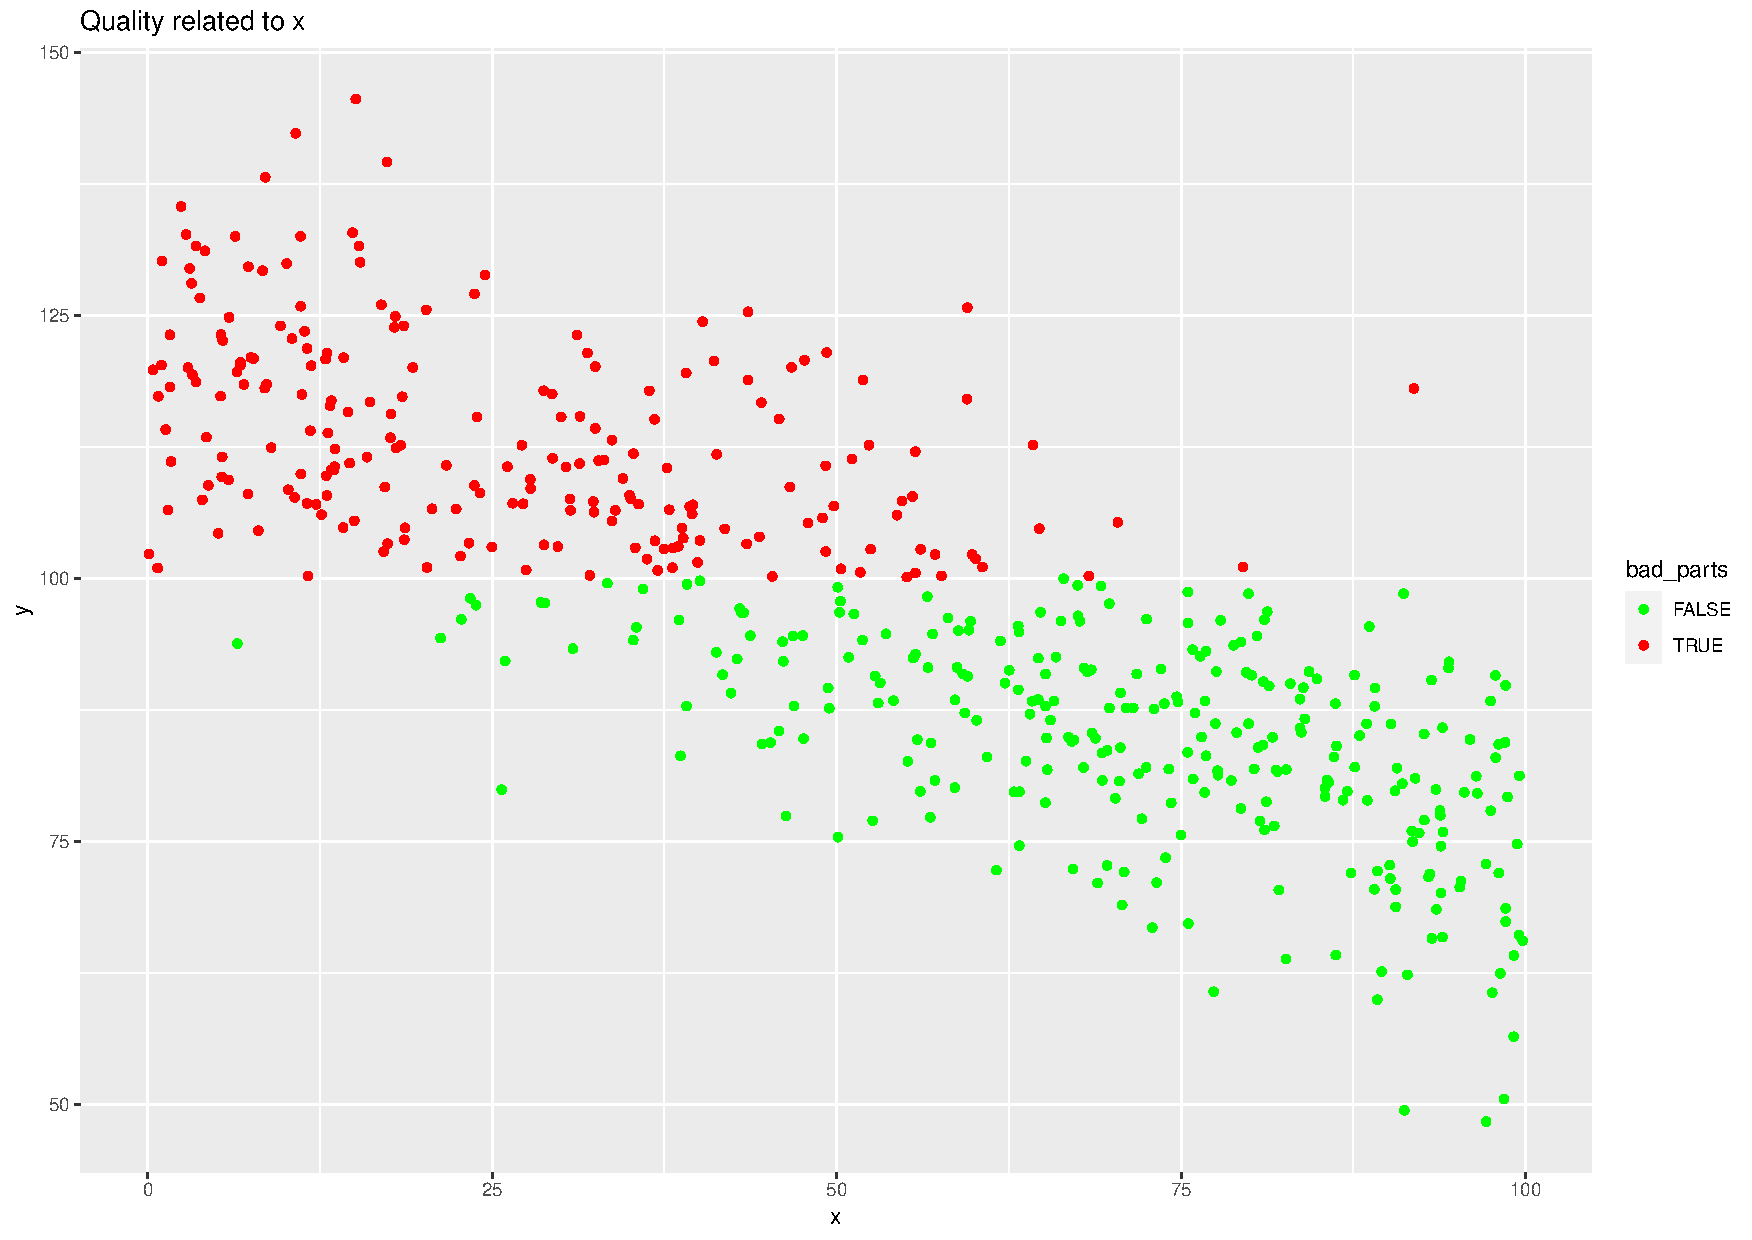
\includegraphics[width=0.95\textwidth]{bad-parts-r.pdf}
	\caption{Diagram of~the distribution of~parts with respect to~the parameter~\emph{x}.}
	\label{fig:bad-parts-r}
\end{figure}

The training sub-sample will~be used to~create a~logistic regression model based on~the values of~the attribute~\emph{x}, which allows you to~assign a~particular part to~quality or~defective. This model will~be used to~assign scores to~the observations in~the training sample. In~the future, these scores will~be used to~construct the ROC curve together with the true labels. Recall that the ROC curve is~plotted for observations with known values of~parameters \emph{x} and~\emph{y}. This ROC curve is~then applied to~the entire set of~objects for which x~values are known but y~values are unknown. The scores themselves as~well as~the~\emph{x} and \emph{y}~values are not displayed on~the graph and are only used for sorting labels. Two different classifiers sorting labels in~the same order will give identical ROC curves regardless of~the absolute values of~the scores. This can~be seen by~constructing an~ROC curve based on~"response" or~"link" predictions from a~logistic regression model. The "response" scores were mapped to~a~(0, 1) scale using a~\href{https://en.wikipedia.org/wiki/Sigmoid_function}{Sigmoid function}\cite{Wiki:sigmoid-function}, the "link" scores were left untransformed. In~this case, the points showing specific observations are ordered in~the same way. To test this hypothesis, we~use the code~\ref{lst:link-response-comparison}. As~you can see in~Figure~\ref{fig:link-response-comparison-r}, the order of~the dots is~the same for "link" and "response".
%
\begin{lstlisting}[float, caption = Comparing "link" and "response" predictions, firstnumber=1, label= lst:link-response-comparison]
fit_glm <- glm(bad_parts ~ x, training_set, family=binomial(link="logit"))

glm_link_scores <- predict(fit_glm, test_set, type="link")

glm_response_scores <- predict(fit_glm, test_set, type="response")

score_data <- data.frame(link=glm_link_scores, 
response=glm_response_scores,
bad_parts=test_set$bad_parts,
stringsAsFactors=FALSE)

score_data %>% 
ggplot(aes(x=link, y=response, col=bad_parts)) + 
scale_color_manual(values=c("green", "red")) + 
geom_point() + 
geom_rug() + 
ggtitle("Both link and response scores put cases in the same order")

\end{lstlisting}
%
\begin{figure}[ht]
	\centering
	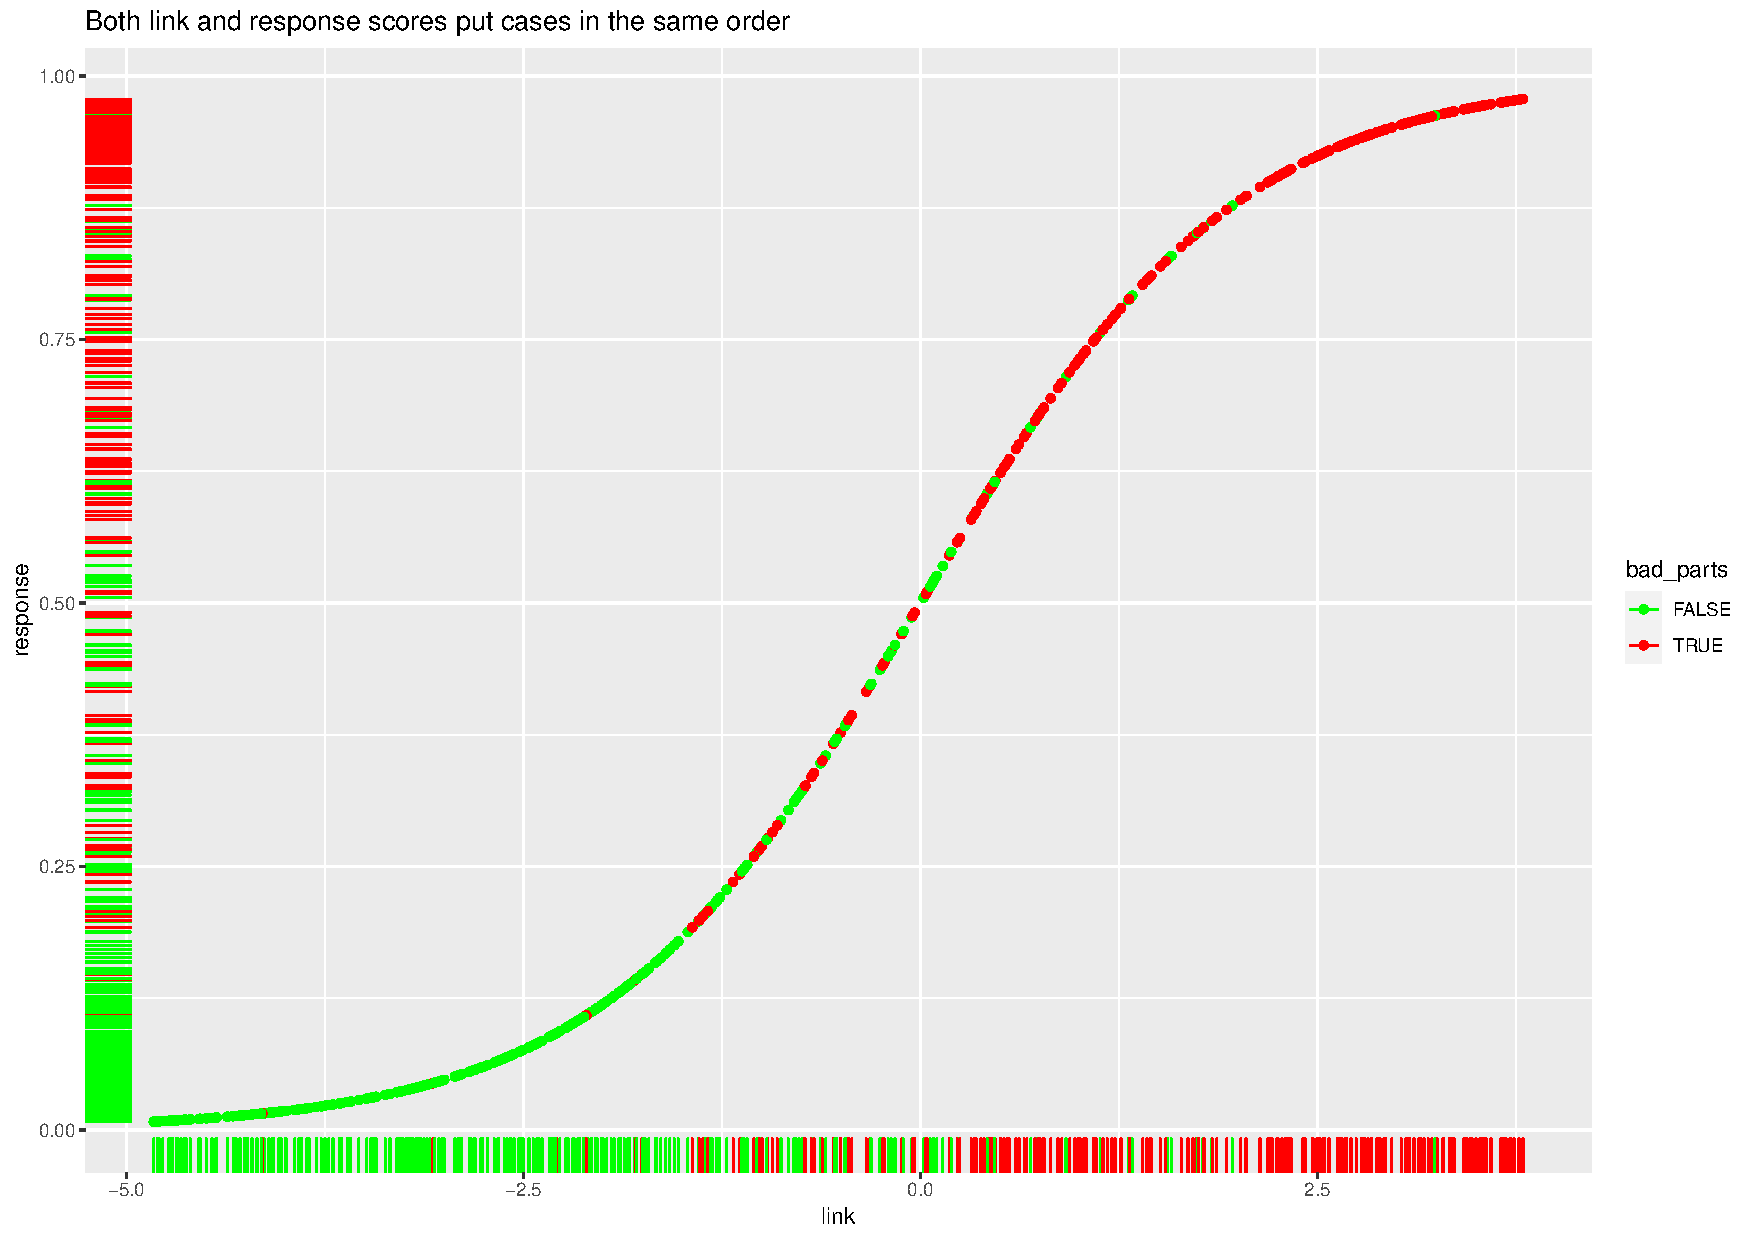
\includegraphics[width=0.95\textwidth]{link-response-comparison-r.pdf}
	\caption{Comparison of~the order of~points for "link" and "response".}
	\label{fig:link-response-comparison-r}
\end{figure}
%

Let's go directly to~the construction of~the ROC curve. We use both the ready function from the "pROC" package and the previously created \textbf{"appraiserRoc"} function (see script~\ref{lst:plot-ROC-1-r}). The result of~the first is~represented as~an~orange curve, the second as~circles of~red for defective parts and black for quality parts (see Diagram~\ref{fig:test-ROC-r}). It~is not difficult to~guess that the red dot corresponded to~the "North" command and the black dot to~the "East" command. Since the library function and the own function perform the same actions, the two curves are identical.

Note that the "Specificity" scale is~plotted on~the abscissa axis, not the FPR, so~the values on~the axis are inverted. Since, according to~Table~\ref{tab:ROC-rates-1}, $"Specificity = 1 - FPR"$ we can talk about the mutual unambiguity of~these indicators. Consequently, when plotting the ROC curve any of~them can~be used. This version of~the scale display was self-selected by~the \textbf{roc} function from the "pRoc" library. If~the user does not set his settings, the function chooses to~display the scale so~that the AUC value is~always greater than 0.5. This calculation is~based on~which group (quality parts, defective parts) has a~higher median score. Since the \textbf{appraiserRoc} function is~of~course not that smart, a~simple subtraction was performed during its use, making it~possible to~build a~joint diagram.

This approach has one limitation: based on~the prognostic nature of~the ordering of~outcomes, it~does not allow correct processing of~information if~the sequence consists of~identical estimates. "Turtle" assumes that the order of~the labels matters, but there is~no~meaningful order in~the situation of~the same scores. These areas should~be displayed with a~diagonal line, but not the traditional steps.
%
\begin{lstlisting}[float, caption = Plotting the ROC curve using library and own functions, firstnumber=1, label= lst:plot-ROC-1-r]
# plot ROC
plot(roc(test_set$bad_parts, glm_response_scores, direction="<"),
col="orange", lwd=3, main="The turtle finds its way", xlim = c(1, 0))
glm_simple_roc <- appraiser_roc(test_set$bad_parts=="TRUE", glm_link_scores)
with(glm_simple_roc, points(1 - FPR, TPR, col=1 + labels))
\end{lstlisting}
%
\begin{figure}[ht]
	\centering
	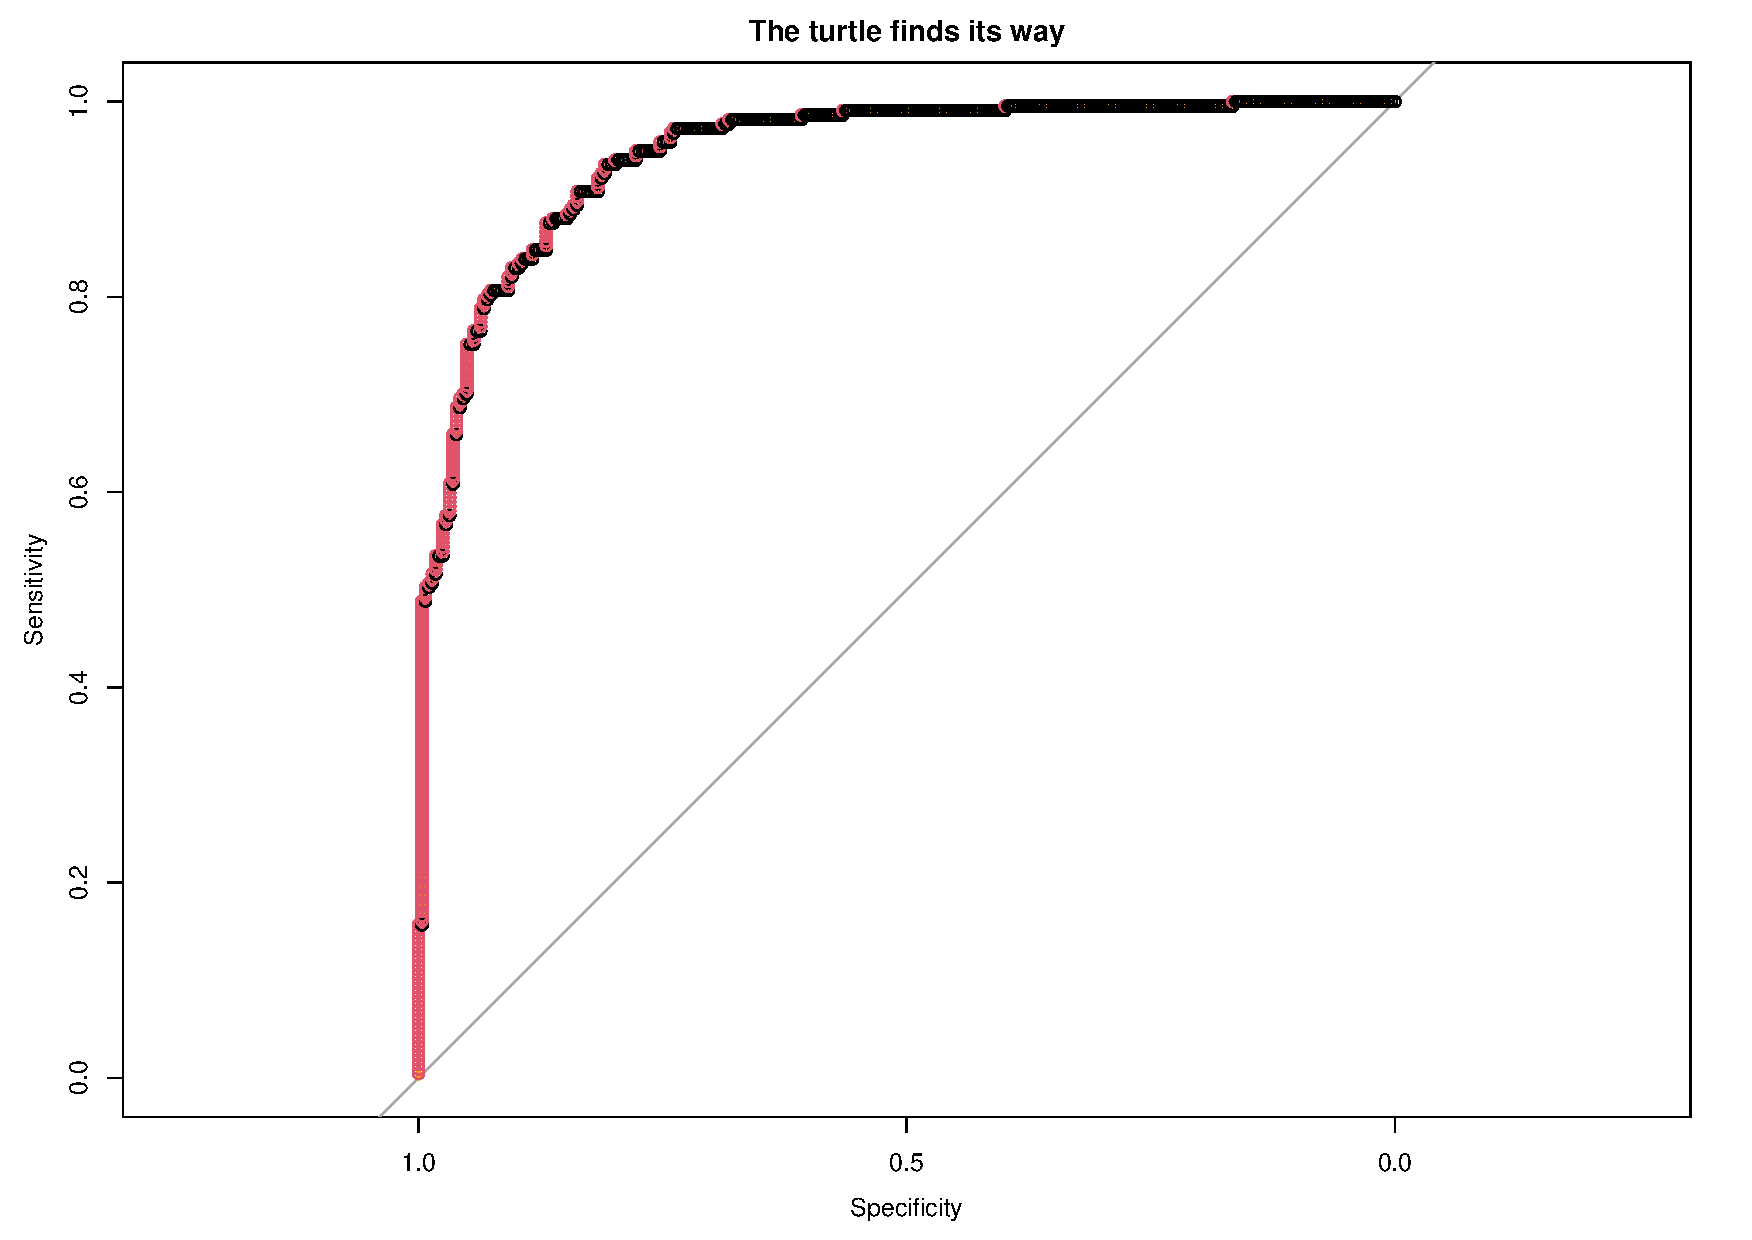
\includegraphics[width=0.95\textwidth]{test-ROC-r.pdf}
	\caption{Identical ROC curves plotted with library and own functions.}
	\label{fig:test-ROC-r}
\end{figure}
%

Consider an~example where a~diagonal is~the only adequate way to~plot a~ROC curve. To~do~this, create an~extremely unbalanced data set in~which only~1\,\% of~the observations are "positive". In~this case, the result of~the prediction will always be~negative. Since all scores will~be the same, there is~no~need for any ordering. The \textbf{roc} function from the "pRoc" package correctly recognizes such situations and draws a~diagonal line~(1,0; 0,1). In~doing so, the turtle assumes that the order of~scores has some significance, and moves between these points along a~random trajectory, alternating between "north" and "east" directions. The code calling the construction of~such a~ROC curve is~given in~script~\ref{lst:plot-ROC-rare-success-r}. In~Diagram~\ref{fig:ROC-rare-success-r}, the black diagonal line was plotted by~the library function, while the blue dashed line was plotted by~our own previously written \textbf{appraiserRoc} function.  As~you can see, the library function correctly determined the case of~identical estimates, while applying our own function resulted in~random turtle wanderings.
%
\begin{lstlisting}[float, caption = Plotting the ROC curve in~case of~absence of~order of~scores, firstnumber=1, label= lst:plot-ROC-rare-success-r]
# plot ROC for 99% negative cases
N <- 2000
P <- 0.01
rare_success <- sample(c(TRUE, FALSE), N, replace=TRUE, prob=c(P, 1-P))
guess_not <- rep(0, N)
plot(roc(rare_success, guess_not), print.auc=TRUE)
appr_roc <- appraiserRoc(rare_success, guess_not)
with(appr_roc, lines(1 - FPR, TPR, col="blue", lty=2))
\end{lstlisting}
%
\begin{figure}[ht]
	\centering
	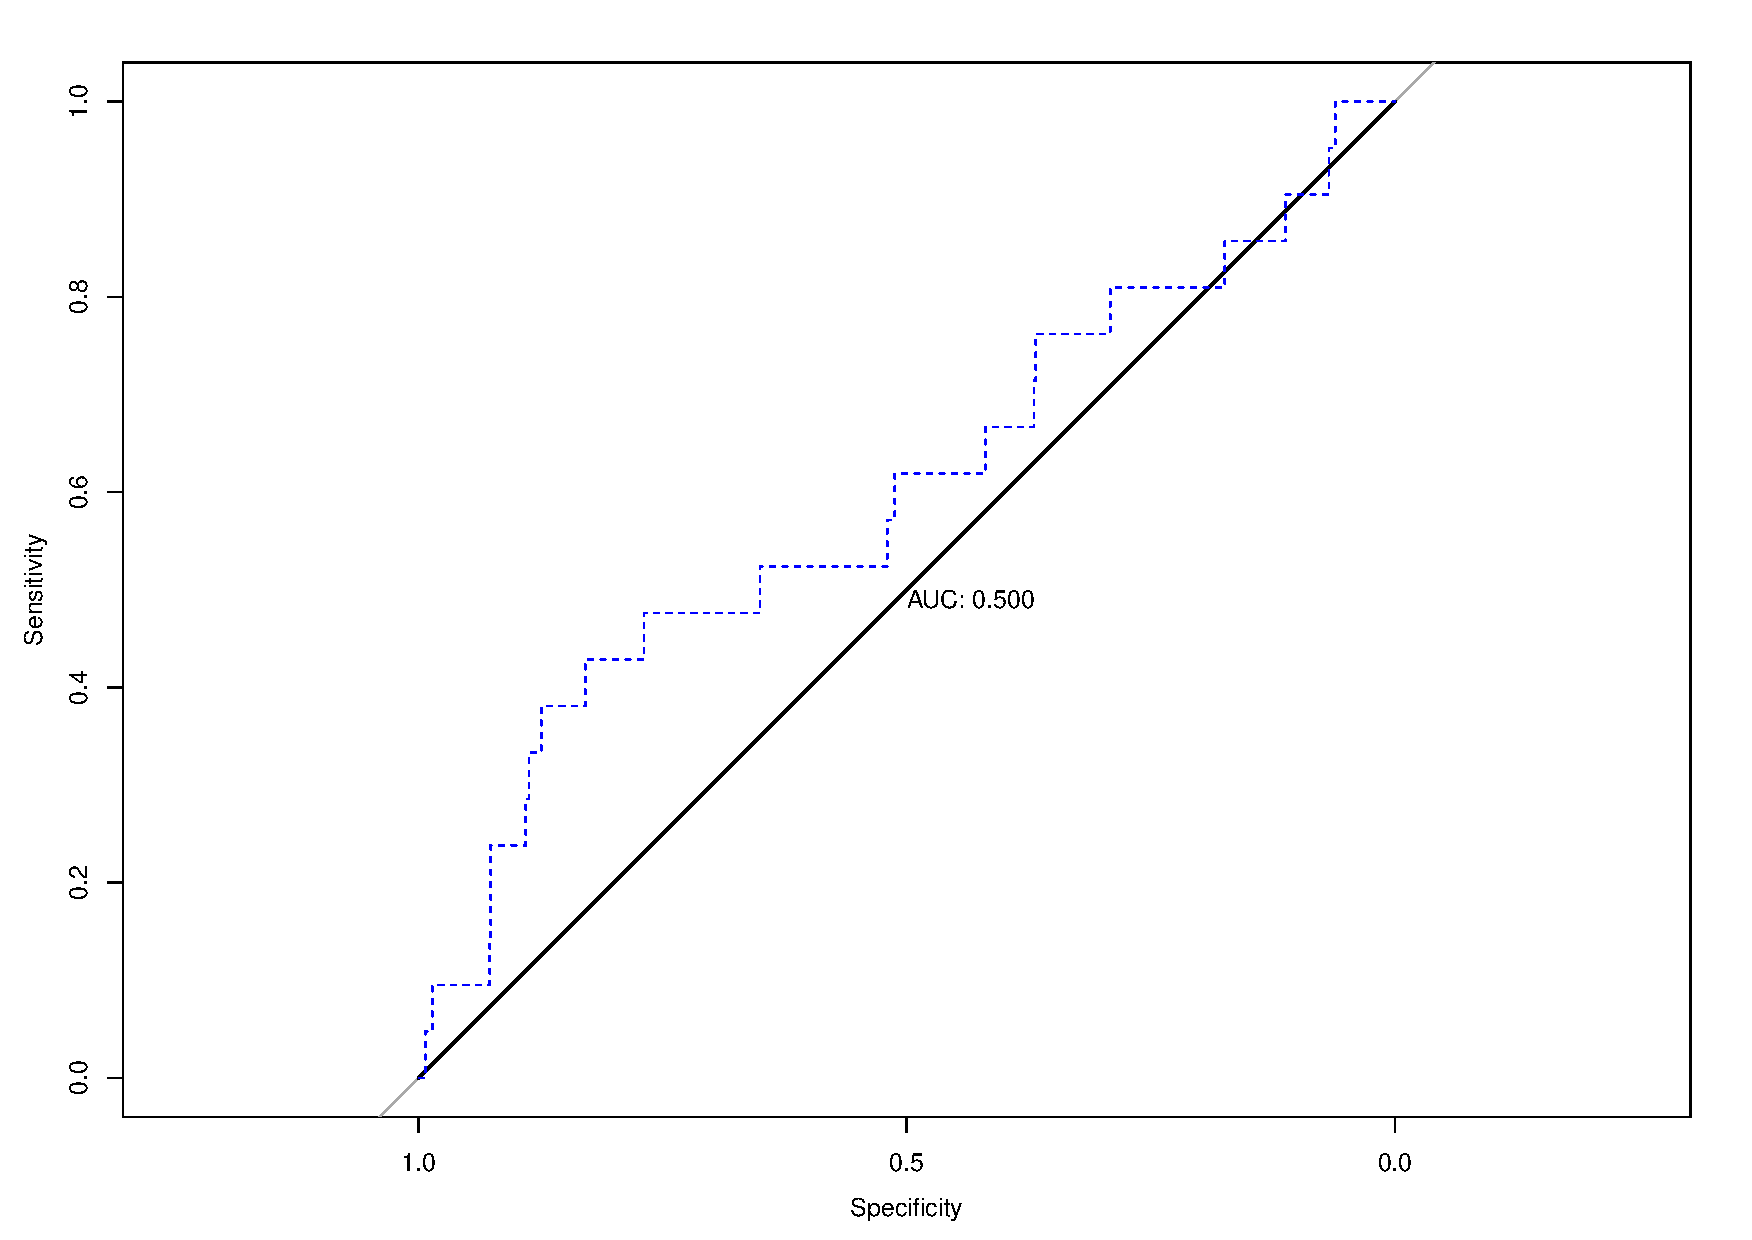
\includegraphics[width=0.95\textwidth]{ROC-rare-success-r.pdf}
	\caption{ROC curve arising when there is~no~value of~the order of~scores.}
	\label{fig:ROC-rare-success-r}
\end{figure}
%

The greater the value of~N, the closer to~the diagonal the turtle will wander. Greater unbalance requires more points in~order for the path to~run roughly close to~the diagonal. In~less extreme cases, the emergence of~diagonal sections is~possible, in~particular, in~the case of~rounding of~estimates, leading to~equality of~some of~them.

To further familiarize yourself with the topic of constructing ROC curves, we can recommend studying this \href{https://web.tresorit.com/l/APSpC#AfkTKO5_-ijMhPuXE-qEzg}{theoretical material}~\cite{ROC-analysis}, as~well as~practice on~the \href{https://kennis-research.shinyapps.io/ROC-Curves/}{online simulator}~\cite{ROC-curve-practice}.
%
\nocite{Essential-Statistical-Inference}
\nocite{AUC-optimization}
\nocite{Mann-Whitney-1947}
\nocite{Optimizing-classifier-performance}
\nocite{ROC-R-1}
\nocite{ROC-AUC-1}
\nocite{ROC-AUC-meets-U-R-1}

\printbibliography
\end{document}          
